\chapter{Methodology}
\label{chap:Methodology}

This section will explain, in detail, the whole process of the proposed methodology, by elaborating, also in a mathematical formulation the problems and the obstacles deriving from the Feature Extraction process and MultiTrack Re-Identification. Furthermore, the pipeline of the proposed methodology will be described in its entirety.

\section{Problem formulation}

\subsection{Feature extraction}
A typical Feature Extraction protocol begins with the formulation of a Vehicle Re-Identification Dataset $\mathcal{X}$, which most often consists of $N$ training images $x_{i} \in \mathbb{R}^{H \times W \times C}$, where $i = 1, 2, ..., N$ and $H, W,$ and $C$ are the Height, Width and Channels of the images, respectively. Each image $x_{i}$ is associated with a unique vehicle identifier $y_{i} \in \mathcal{Y}$ where $\mathcal{Y}$ represents a finite set of labels \textit{(e.g. $\mathcal{Y} = {1, 2, ... \, M}$)} for $M$ unique vehicles. This particular set will be referred as the Training Set:
\[
    \mathcal{X}_{train} = \{(x_i, y_i) \mid i = 1, 2, \ldots, N\},
\]

The evaluation procedure is performed on a Test Set, denoted as $\mathcal{X}_{test}$, which does not intersect with the training set and is divided into two disjoint subsets: gallery $\mathcal{G}$ and query $\mathcal{Q}$. The gallery set $\mathcal{G}$ consists of a collection of $P$ images $g_{i} \in \mathcal{G}$, each corresponding to one or more vehicles:
\[
    \mathcal{G} = \{(g_k, y_k) \mid k = 1, 2, \ldots, P\}
\]

Meanwhile, the query set $\mathcal{Q}$ is made up of $Q$ images $q_{j} \in \mathcal{Q}$, each representing a vehicle that needs to be matched to its corresponding entry in the gallery $\mathcal{G}$:
\[
    \mathcal{Q} = \{(q_j, y_j) \mid j = 1, 2, \ldots, Q\}
\]

Thus, the Test Set can be expressed as the union of those two:
\[
    \mathcal{X}_{test} = \mathcal{Q} \cup \mathcal{G}, \text{ where } \mathcal{Q} \cap \mathcal{G} = \emptyset
\]

Finally, the entire Dataset can be represented as a set of image-label pairs:

\begin{equation}
    \begin{aligned}
        \mathcal{X} & = \{\mathcal{X}_{train} \cup \mathcal{X}_{test}\}\\
                    & = \{\mathcal{X}_{train} \cup \mathcal{Q} \cup \mathcal{G}\}
    \end{aligned}
  \end{equation}

The goal of vehicle re-identification is to learn a mapping function 
\[
    f : \mathbb{R}^{H \times W \times C} \to \mathbb{R}^d,
\] 
characterized by some parameters \(\theta\), such that for an Image \(x \in \mathbb{R}^{H \times W \times C}\), the function outputs a feature vector \(v_{x} = f(x; \,\theta) \in \mathbb{R}^d\). As in an usual Deep Learning methodology, the final solution is achieved by optimizing of the parameters \(\theta\), along with the consequent minimization of a loss function \(\mathcal{L}\) that measures the discrepancy between the predicted feature vectors and the actual ground truth labels:
\[
    \theta^{*} = \argmin_{\theta} \mathcal{L}(f(x; \,\theta)),
\]

In order to do so, those feature vectors are, then, further optimized in such a way that a predefined distance metric 
\[
    d: \mathbb{R}^d \times \mathbb{R}^d \to \mathbb{R}_{\geq 0}
\]
satisfies the following properties:
\begin{itemize}
    \item \(d(v_{x_i}, v_{x_j})\) is small if \(x_i\) and \(x_j\) belong to the same vehicle (\(y_i = y_j\)).
    \item \(d(v_{x_i}, v_{x_j})\) is large if \(x_i\) and \(x_j\) belong to different vehicles (\(y_i \neq y_j\)).
\end{itemize}

This framework ensures that feature vectors are discriminative and facilitate effective vehicle re-identification.

\subsection{MultiTrack Re-Identification}
In a MultiTrack Re-Identification (Re-ID) problem, the goal is to associate vehicle tracklets observed from multiple cameras into consistent trajectories representing the same vehicle. Let us define the set of $T$ tracklets extracted from multiple cameras as:
\[
    \mathcal{T} = \{T_k \mid k = 1, 2, \ldots, T\},
\]
where each tracklet $T_k$ is a sequence of bounding boxes $B_{k, i}$ from frames $i = 1, 2, \ldots, n_k$, with $n_k$ denoting the number of frames within the $k$-th tracklet. Formally:
\[
    T_k = \{B_{k, i} \mid i = 1, 2, \ldots, n_k\}.
\]

Each tracklet $T_k$ is associated with a feature representation $v_k \in \mathbb{R}^d$, which is obtained by aggregating the feature vectors of its constituent bounding boxes using a pooling strategy (e.g., Mean or Max Pooling):
\[
    v_k = \text{Aggregate}(\{f(B_{k, i}; \,\theta) \mid i = 1, 2, \ldots, n_k\}).
\]

The MultiTrack Re-ID challenge seeks to determine which tracklets in $\mathcal{T}$ correspond to the same vehicle by learning a similarity function $S: \mathbb{R}^d \times \mathbb{R}^d \to \mathbb{R}$ that satisfies the following criteria:
\begin{itemize}
    \item $S(v_k, v_l)$ assumes a high value when $T_k$ and $T_l$ belong to the same vehicle.
    \item $S(v_k, v_l)$ takes a low value if $T_k$ and $T_l$ belong to different vehicles.
\end{itemize}

The task is, then, to group these tracklets into a set of disjoint clusters, $\{\mathcal{C}_m \mid m = 1, 2, \ldots, M\}$, where each cluster $\mathcal{C}_m$ represents all tracklets belonging to the same vehicle. This can be expressed as:
\[
    \mathcal{C}_m = \{T_k \in \mathcal{T} \mid y_k = y_m\},
\]
where $y_k$ and $y_m$ denote the unique vehicle IDs associated with tracklets $T_k$ and $T_m$, respectively. Clustering is typically performed by either trying to minimize a distance function (like Euclidean distance) or trying to maximize a similarity function (like Cosine Similarity)

The MultiTrack Re-ID challenge can thus be framed as an optimization problem to obtain the similarity function $S$ that clusters tracklets of the same vehicle together, while keeping tracklets from different vehicles far apart, enabling the implementation of an accurate Multi-Camera Multi-Track (MTMC) Re-ID system.

\section{Pipeline}
In the Feature Extraction step, the pipeline defines and trains a Convolutional Neural Network (CNN) model for Vehicle Re-Identification and applies clustering methods for the MultiTrack Re-ID step. Model training involves several techniques in the scope of Loss Functions, Dataloader Sampling, and Learning Rate Scheduling, along with Data Augmentation and different model architectures. An overview of the pipeline is shown in Figure \ref{fig:PipelineOverview}.

\subsection{Network Architecture}
In the Network Architecture phase, several tricks and techniques are adopted to improve the performance of the standard CNN model. They are listed as follows:

\subsubsection{Backbone}
\label{subsubsec:Backbone}
The backbone of the model is a Convolutional Neural Network (CNN) that extracts features from the input images. It is also responsible for learning visual representations of the vehicles, which are further used in computing the similarity between the vehicles. The backbone used for this project varies between the vanilla ResNet family and their IBN (Instance Batch Normalization) variants \cite{IBN-Net} as shown in Figure \ref{fig:ResNetBNNeck} and Figure \ref{fig:IBNLayer}, which have shown to be effective in learning discriminative features for Re-ID tasks since the Feature Extractor can learn robust encoded representations that are invariant to appearance differences \cite{StrongBaselineForVehicleReID} as shown also by the activation maps in \ref{fig:ActivationMaps}. Secondly, It is also capable of enhancing the performances of various state-of-the-art Deep Neural Network models like ResNet, ResNeXt and SENet.

% ResNet Architecture and IBNLayer Image
\begin{center}
    \begin{figure}[t]
        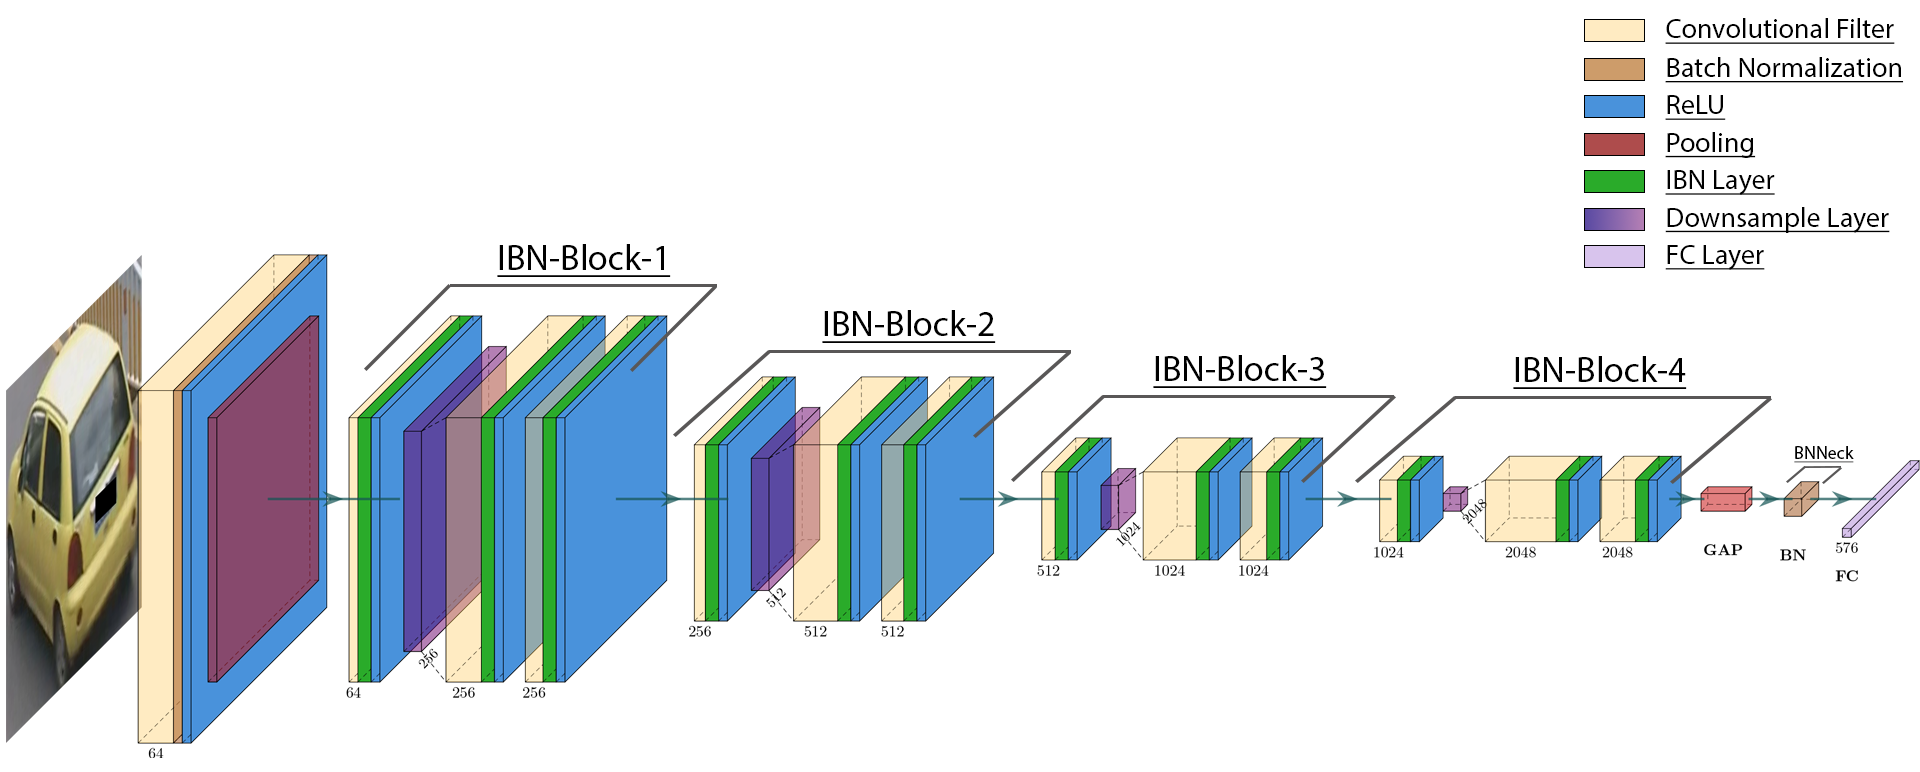
\includegraphics[width=0.90\textwidth]{images/ResNetFinalArchitecture.png}\hfill
        \caption[ResNet-IBN-50 Architecture with BNNeck]{ResNet-IBN-50 architecture with BNNeck}
        \label{fig:ResNetBNNeck}
        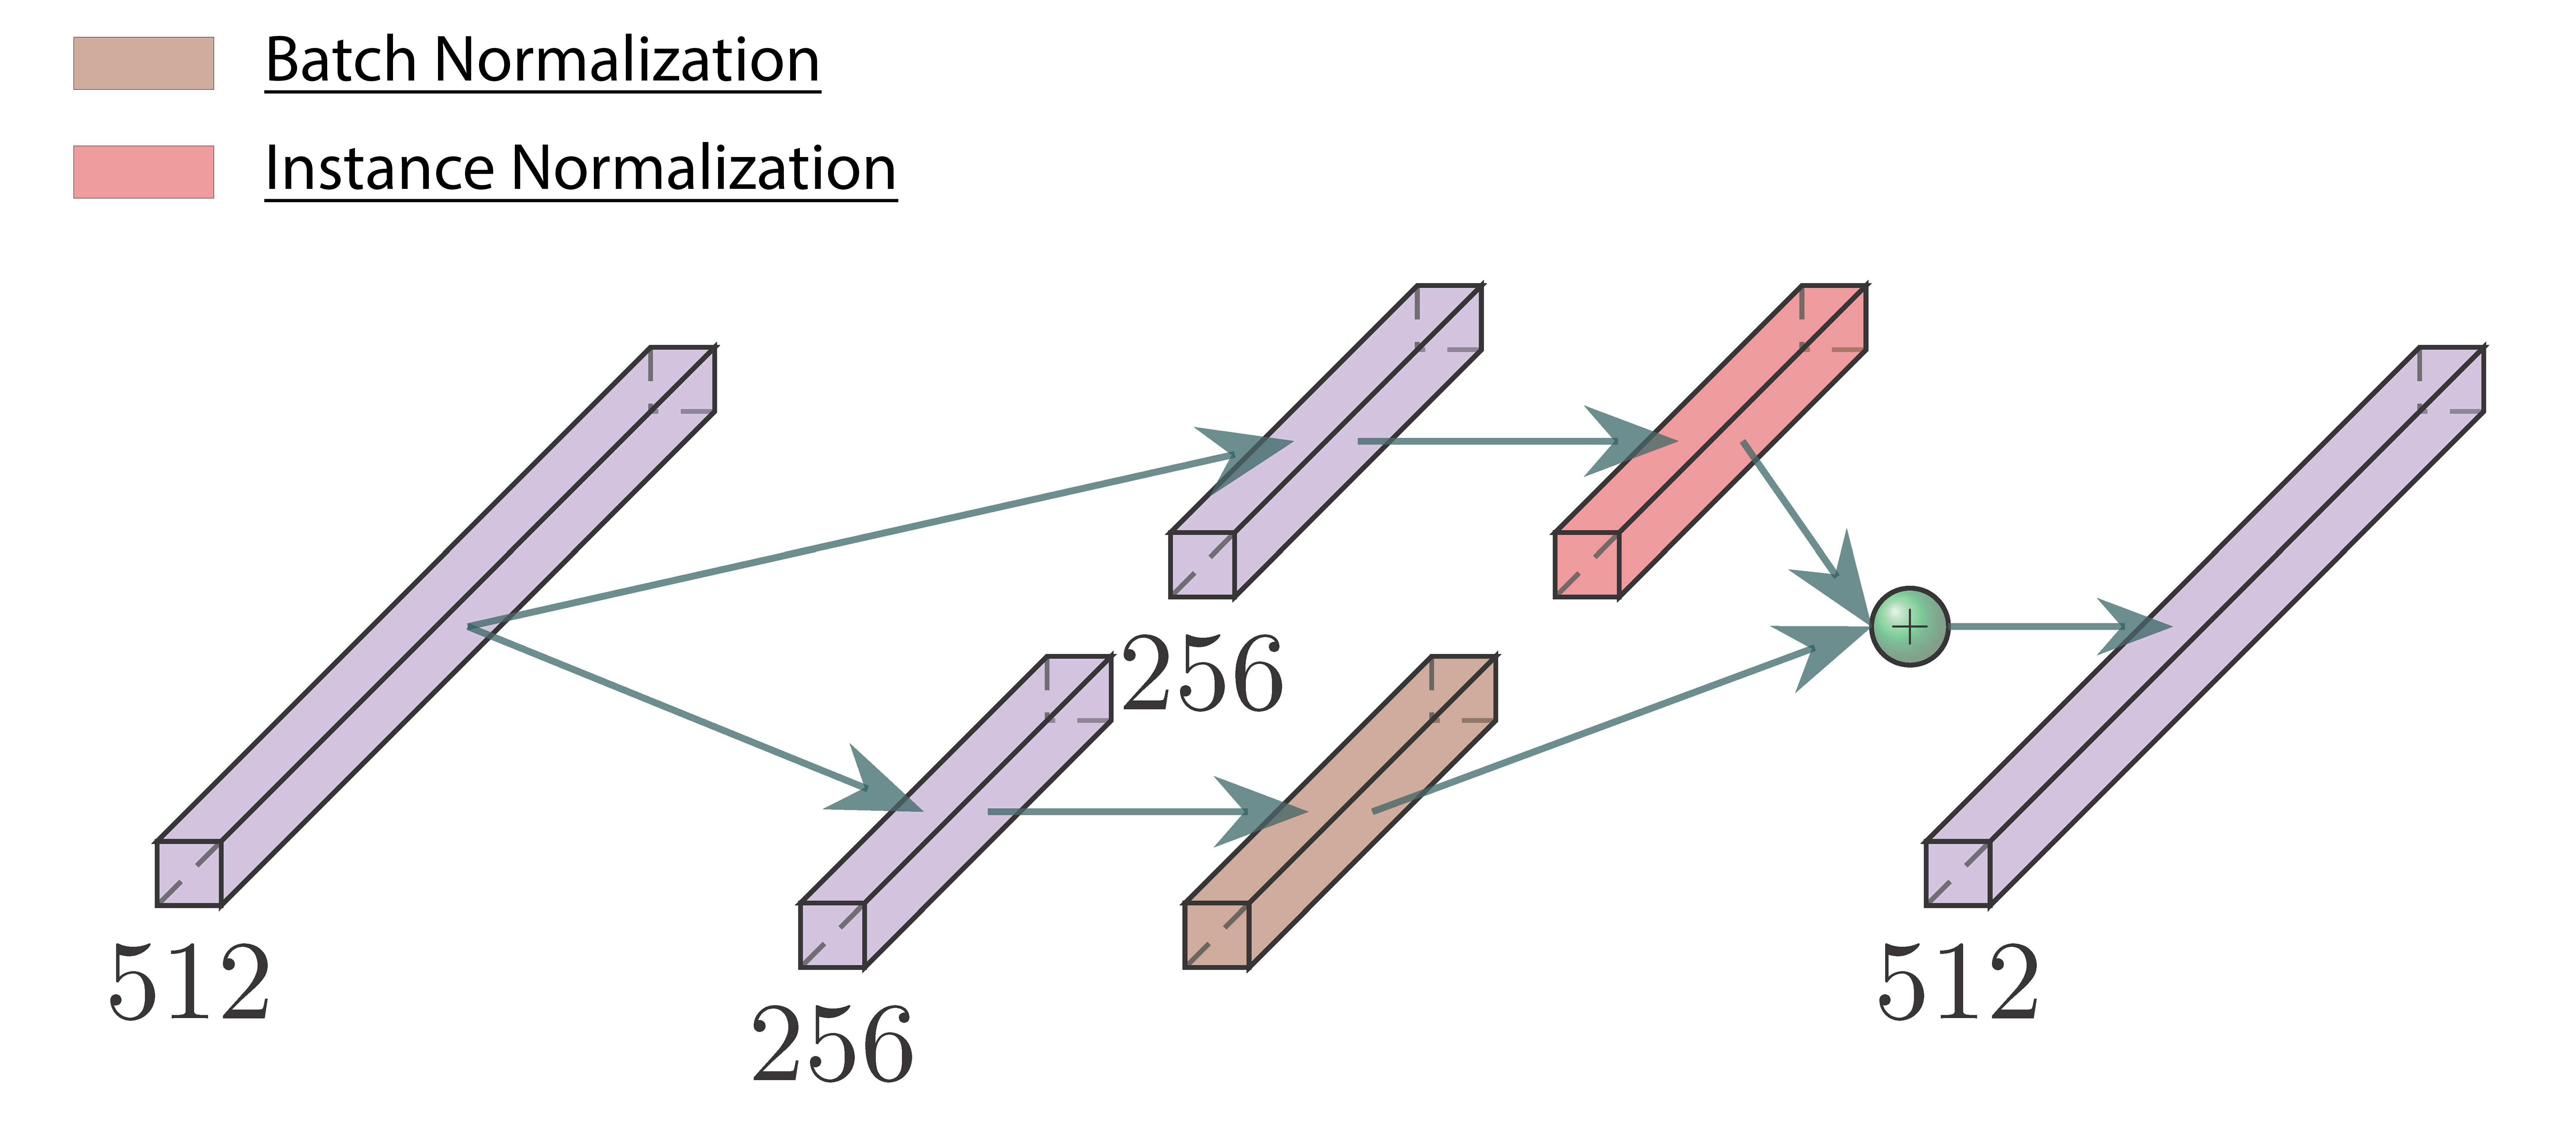
\includegraphics[width=0.90\textwidth]{images/IBNLayer.png}\\
        \caption[IBN (Instance Batch Normalization) Layer in detail]{An IBN (Instance Batch Normalization) Layer in detail}
        \label{fig:IBNLayer}
    \end{figure}
\end{center}

% Activation Maps
\begin{figure}[H] 
    \centering
    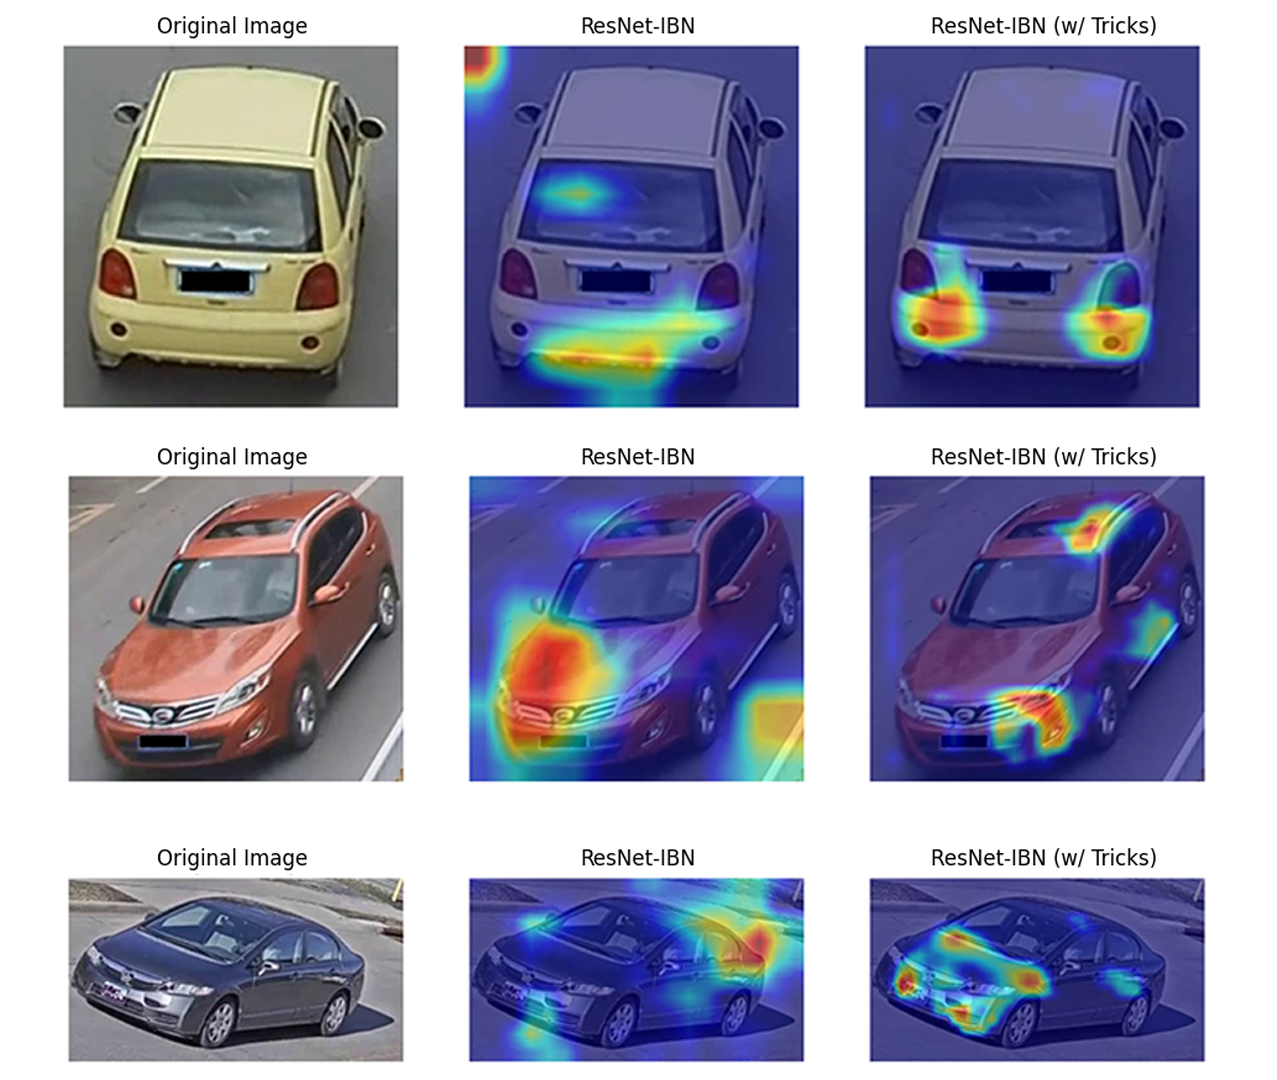
\includegraphics[width=0.60\textwidth]{images/ActivationMaps2.png}
    \caption[Activation Maps for ResNet-IBN]{Activation Maps of the ResNet-IBN-50 Backbone using GradCAM. Middle frame represents the Vanilla IBN model, while the right frame represents the IBN model with BNNeck trained on Re-ID Datasets. The activation maps show that the model focuses on specific car body parts, like roof, rear lights or front hood of the vehicle, which are crucial for Vehicle Re-ID tasks.}
    \label{fig:ActivationMaps}
\end{figure}

\subsubsection{Stride}
\label{subsubsec:Stride}
The last spatial down-sampling operation in the backbone network is referred to as the final stride, and for the ResNet50 backbone, it is fixed to $2$. Basically, when fed into an image with 256$\times$128 size, it outputs a feature map with a spatial size of (8$\times$4). If last stride is changed from 2 to 1, then we can obtain a feature map with increased spatial size (16$\times$8). This manipulation only slightly increases the computation cost and does not involve extra training parameters. However, an increased spatial resolution brings significant improvement, hence the stride parameter in the last Convolutional Layers is set to 1, which means that the Convolutional Filters move one pixel at a time. This is performed to maintain the spatial resolution of the input image, which is important in the Vehicle Re-ID task because it lets the model extract more detailed features from the input images \cite{StrongBaselineBatchNorm}.

\subsubsection{GeM Pooling}
\label{subsubsec:GeMPooling}
The Global Adaptive Average Pooling (GAAP) layer is replaced by the Generalized Mean Pooling (GeM) layer \cite{GeMPooling, FastReID}, which is proven to be effective in extracting unique features related to Re-ID tasks. The GeM Pooling layer is used to aggregate the feature maps from the backbone network into a single feature vector, which is then used to compute the similarity between the vehicles. The aggregation layer is designed to condense the feature maps produced by the backbone into a single global feature vector. This pooling layer takes as input a tensor $\mathbf{X} \in \mathbb{R}^{W \times H \times C}$, where $W$, $H$, and $C$ represent the width, height, and channel dimensions of the feature maps, respectively. The resulting global feature vector $\mathbf{f} \in \mathbb{R}^{1 \times 1 \times C}$ achieved by an aggregation operation.

The global feature vector $\mathbf{f} = [f_1, f_2, \dots, f_C]$ is obtained using the following pooling methods:

\begin{enumerate}
    \item \textbf{Adaptive Average Pooling}: Computes the mean value across all spatial locations for each channel:
    \begin{equation}
    f_c = \frac{1}{|\mathbf{X}_c|} \sum_{x \in \mathbf{X}_c} x
    \end{equation}

    \item \textbf{GeM Pooling}: Generalized Mean Pooling applies a power operation followed by the mean and root, controlled by the parameter $\alpha$:
    \begin{equation}
    f_c = \left( \frac{1}{|\mathbf{X}_c|} \sum_{x \in \mathbf{X}_c} x^\alpha \right)^{\frac{1}{\alpha}}
    \end{equation}
\end{enumerate}

Here, $|\mathbf{X}_c|$ is the number of spatial locations in channel $c$ and $\alpha$ is a control parameter for GeM pooling.

\subsection{Batch Normalization Neck (BNNeck)}
\label{subsec:BNNeck}
The Batch Normalization Neck (BNNeck) \cite{StrongBaselineBatchNorm} is a method to enhance the performance of ReID models by adding a Batch Normalization (BN) layer in the gap between the extracted feature vectors and the classifier layers. to alleviate the conflicts arising from the combination of Identity (ID) Loss and Triplet Loss in the training process.

As shown in \cite{StrongBaselineBatchNorm}, many state-of-the-art methods use both ID and triplet losses to supervise the same feature vector. This combination generally improves model performance. However, these two losses operate under different principles in the embedding space, leading to potential conflicts. ID loss divides the embedding space into subspaces by hyperplanes, where features in each class subspace are distributed affinely. Hence, cosine distance is a more suitable choice than Euclidean distance during inference for models optimized by ID loss. On the other hand, triplet loss encourages intra-class compactness and inter-class separability in Euclidean space and thus it opearates on feature clusters.

Using both losses simultaneously will cause a conflict because the optimization targets are inconsistent. During training, one loss could outweigh the other one or they both could fluctuate, as observed in \cite{StrongBaselineBatchNorm}. For this reason, there exists a mutual interaction: the ID loss dictates the intra-class compactness motivated by Triplet loss, and conversely, Triplet loss disrupts and fragments the clear decision boundaries of the ID loss, resulting in a non-optimal "tadpole-shaped" feature distribution, hence while such a direct combination of these two losses boosts the performance, better alternatives exist for it.

To address this problem, Xiong et al. \cite{StrongBaselineBatchNorm} inserted a Batch Normalization (BN) layer between the feature extraction stage, e.g., GeM Pooling, and the classifier layers as shown in Figure \ref{fig:ResNetBNNeck}. This BN layer not only reduces overfitting but also smooths the distribution of features in the embedding space.  During training, the features before the BN layer ($f_{Trip}$) are used for the Triplet Loss, and the features after the BN layer ($f_{ID}$) are used for the ID loss. This separation allows $f_{Trip}$ to keep a compact distribution while $f_{ID}$, benefiting from ID supervision, forms clear decision boundaries. More in detail, for the ID loss, it improves intra-class compactness by pulling features closer to the center of their respective subspaces, which improves the model's ability in class separation and, for triplet loss, BN increases the intra-class feature radius by tightening its decision boundaries. During inference, $f_{Trip}$ is calculated immediately following the BN layer this time and is applied to the Vehicle ReID task with a metric of cosine similarity, as it performs better than Euclidean distance. All this is visualized in Figure \ref{fig:Losses}.

% Losses Image
\begin{figure}[H]
    \centering
    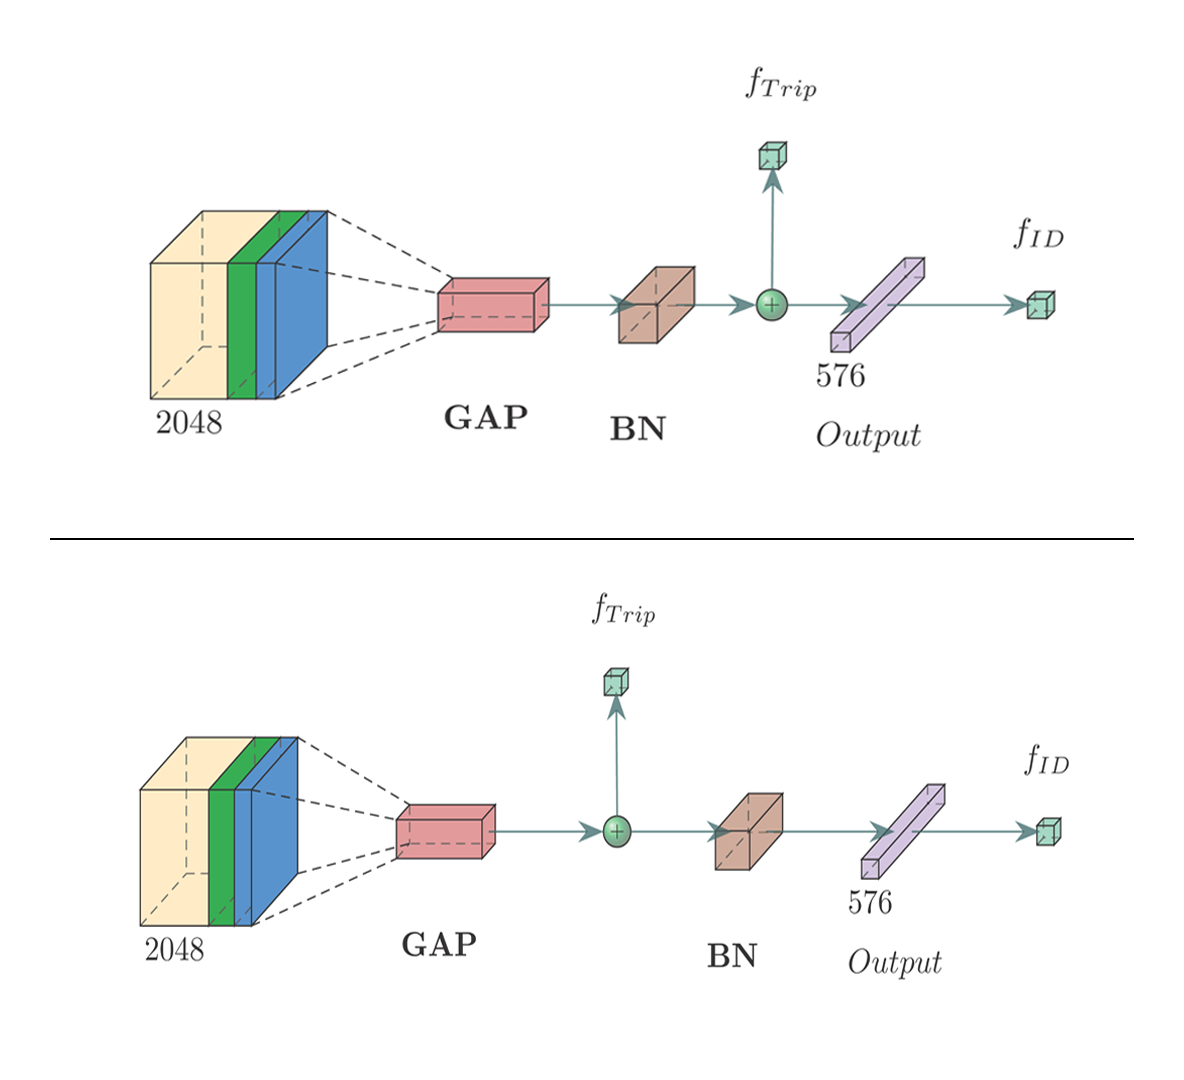
\includegraphics[width=0.80\textwidth]{images/Losses.png}
    \caption[Training and Inference representation]{Representation of the feature vectors during Training (top) and Inference (bottom) in the BNNeck architecture. The feature vectors $f_{ID}$ and $f_{Trip}$ are used for ID and Triplet Losses, respectively.}
    \label{fig:Losses}
\end{figure}

Experimental results from \cite{StrongBaselineBatchNorm} have proven the effectiveness of BNNeck by showing a substantial improvement in ReID performance, guaranteeing a good optimization balance, contrary to the overall inconsistencies between ID and Triplet losses.

% \subsubsection{Glamor Training}
% The training process presented in this work \cite{Glamor} employs Group Normalization (GN) Layers instead of Batch Normalization (BN) Layers as integral components of the architecture, replacing the Batch Normalization (BN) layers present in the IBN ResNet variant. Also, as for the ID Loss, the embeddings $f$ are passed through a Layer Normalization (LN) window, applied specifically before the softmax operation. These normalization techniques are used to stabilize the training process and enhance the model's convergence. By normalizing features within the network, GN and LN mitigate issues related to parameter initialization sensitivity and help maintain consistent performance even in scenarios with smaller batch sizes. The combination of GN and LN ensures that the embedding space is properly aligned for downstream tasks, with improved stability during optimization.

% Overall, this training strategy highlights the utility of applying normalization layers directly within the architecture, particularly in combination with other network components, to refine feature embeddings. This approach enhances the model's ability to generalize across different conditions, providing a more effective solution for tasks such as vehicle re-identification.

\subsection{Loss Functions}
\label{subsec:LossFunctions}
In order to train the Re-ID model, as explained in the previous subsection, a two-fold loss strategy is implemented, combining ID Loss and Metric Loss. The first improves class separation by making the predictions sharper toward the correct class labels, and the latter guarantees that the vehicles with very similar visual appearances are mapped closer to each other in the embedding space. This combination is able to generate very specific discriminative and generalized features necessary in the vehicle re-identification task.

\subsubsection{ID Loss}
The ID loss is applied in Re-ID tasks by using \textbf{Cross Entropy Loss} (CE), which is a common loss function for classification tasks. It is used to optimize the model's predictions to match the true class labels, encouraging classes to be well separated in the learned representation. In another hand, by using soft targets which are a weighted average of the hard targets and the uniform distribution over labels, prevents the network from becoming over-confident and so more robust. Smoothing the labels in this way means using CrossEntropyLoss with Label Smoothing \cite{LabelSmoothing, LabelSmoothing2}. Given the true labels $y_{k}$ and the predicted probabilities $p_{k}$, for each class $k$, the ID Loss is defined as:

\[
    \mathcal{L}_{\text{\textit{ID}}} = \sum_{k=1}^{K} - y_{k}^{\textit{LS}} \cdot \log (p_{k})
\]

where:
\begin{itemize}
    \item $y_{k}^{LS} = y_{k} \cdot (1-\beta) + \beta / K$ \textit{(label smoothing)},
    \item $K$ is the number of classes,
    \item $p_{k}$ is the predicted probability for class $k$.
\end{itemize}

\subsubsection{Metric Losses}
The training involves two types of Metric Losses, namely \textit{Triplet Loss} and \textit{Supervised Contrastive Loss}, both of which originate from the concept of Contrastive Learning. This could be interpreted in such a way that one trains the model to minimize the distances between samples of the same class label, keeping them close in the embedding space, while increasing the distances between samples of different classes in order to separate them properly in the final learned representation.

Specifically, the \textbf{Triplet Loss} \cite{TripletLoss, TripletLossV2} is used to have some control over the structure that shall be imposed onto the embedding space. For a Dataset $\mathcal{D}$ containing a given anchor input $x$, the aim here is to minimize the distance between the anchor and positive samples ($x^{+}$) while maximizing it between the anchor and negative samples ($x^{-}$), like in Figure \ref{fig:TripletLoss}. Here, the positive samples are those of the same class as the anchor sample, while negative ones are from different classes. The Triplet Loss is, then, defined as:
\[
    \mathcal{L}_{\textit{Triplet}}(x, x^{+}, x^{-}) = \sum_{x \in \mathcal{D}} \max({0, \left\Vert\left(f(x) - f(x^{+})\right) \right\Vert^2} - \left\Vert\left(f(x) - f(x^{-})\right) \right\Vert^2 + \alpha),
\]

where $\alpha$ is the margin value or minimum offset between distances of similar and dissimilar pairs of samples.

% TripletLoss Image
\begin{figure}[ht]
    \centering
    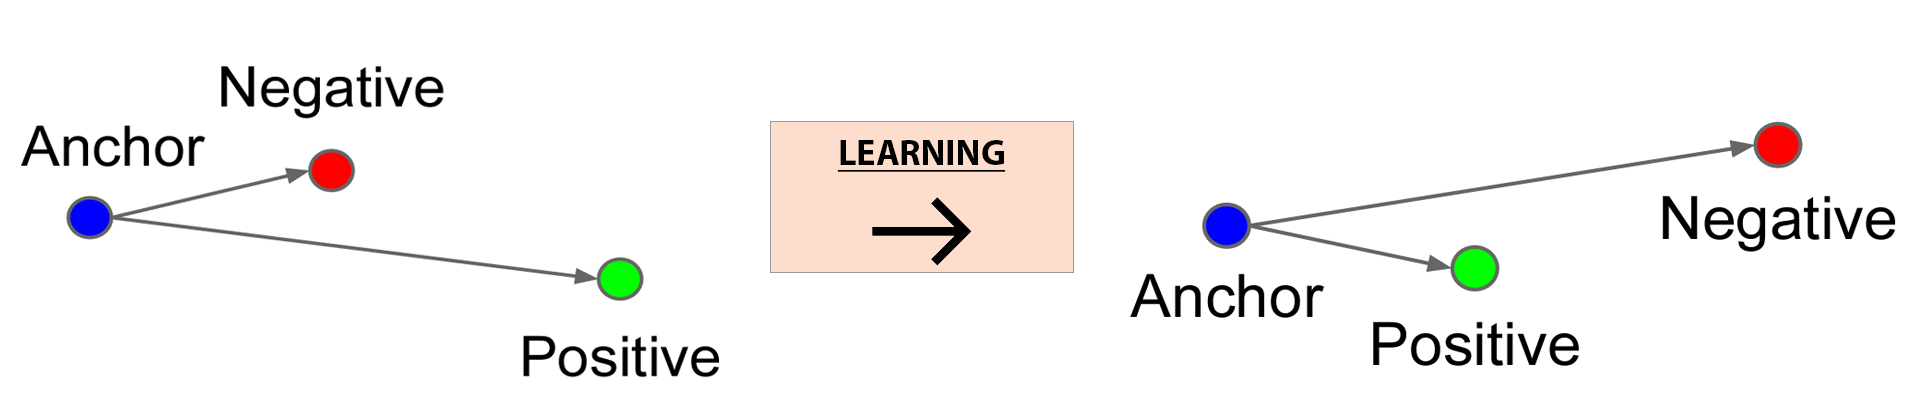
\includegraphics[width=1.0\textwidth]{images/TripletLoss.jpg}
    \caption[A Triplet Loss illustration]{Illustration of Triplet Loss given one positive and one negative sample per anchor}
    \label{fig:TripletLoss}
\end{figure}

\textbf{Supervised Contrastive Loss} \cite{SupConLoss} is an extension of Contrastive Learning, which is specifically designed for the Supervised setting. On the other hand, unlike Triplet Loss, which considers one positive and one negative example related to every anchor, SupCon Loss considers multiple positive and negative examples related to every anchor. For a dataset $\mathcal{D}$, it pulls together the embeddings of samples belonging to the same class while pushing them apart from the embeddings of other classes, hence achieving a robust class-clustering in the embedding space.

Formalizing, let $N$ denote the number of samples in a batch and $P(i)$ the set of positive samples for an anchor $i$ within a multiviewed batch. SupCon Loss over a batch can now be expressed as:
\[
    \mathcal{L}_{\textit{SupCon}} = \frac{1}{N} \sum_{i=1}^N \frac{-1}{|P(i)|} \cdot \sum_{p \in P(i)} \log \frac{\exp\left( \frac{z_i \cdot z_p}{\tau} \right)}{\sum_{a \in A(i)} \exp\left( \frac{z_i \cdot z_a}{\tau} \right)},
\]
where:
\begin{itemize}
    \item $z_i, z_p, z_n$ denote the normalized embeddings of the anchor $i$, positive $p$, and negative $n$ samples,
    \item $A(i)$ is defined as the set of all samples in the batch excluding $i$,
    \item $P(i)$ a set of all positive samples to anchor $i$,
    \item $|P(i)|$ indicates is the number of positive samples for anchor $i$,
    \item $\tau$ is a temperature parameter to control the separation margin.
\end{itemize}

Compared to the Triplet Loss, SupCon Loss works without hard negative mining and is generally much more stable while training. This is due to the fact that it uses all positive samples of a class and not just one positive-negative pair, hence it tends to get optimized way faster. Thus, SupCon Loss often leads to better embedding clustering and higher robustness during hyperparameter search.

Finally, the overall Re-ID loss is expressed as:
\[
    \mathcal{L}_{\textit{ReID}} = \mathcal{L}_{\textit{ID}} + \mathcal{L}_{\textit{Metric}},
\]

where $\mathcal{L}_{\textit{Metric}}$ could either be $\mathcal{L}_{\textit{Triplet}}(\cdot)$ or $\mathcal{L}_{\textit{SupCon}}(\cdot)$. 

\subsubsection{Momentum Adaptive Loss Weight (MALW)}
Following \cite{StrongBaselineForVehicleReID}, the MALW scheme (as in \ref{fig:MALW}) updates dynamically the weights of $\mathcal{L}_{\textit{ID}}$ and $\mathcal{L}_{\textit{Metric}}$ dynamically during training. Although a conventional 1:1 weighting is widely adopted, this often leads to an imbalance, since $\mathcal{L}_{\textit{ID}}$ often has a larger magnitude that dominates $\mathcal{L}_{\textit{Metric}}$. This may affect the efficiency of training, and manually tuning the weights is both time-consuming and suboptimal.

MALW addresses this by automatically balancing the contribution of the two losses with respect to their statistical properties, such as standard deviation. This adaptive mechanism allows the model to prioritize each loss appropriately throughout the training process.
Both terms, \(\lambda_{\textit{ID}}\) and \(\lambda_{\textit{Metric}}\), are initialized to be the same in value for both losses. In contrast, \(\lambda_{\textit{ID}}\) (ID Weight) is updated every \(K\) iterations with the help of a momentum factor on the moving average of the measured loss values, so that updates are gradually and progressively and stable.

Because the network cannot be dominated by any of the components of loss, MALW allows for better optimization dynamics and hence achieves much better convergence and therefore good performance.

% MALW Image
\begin{figure}[H]
    \centering
    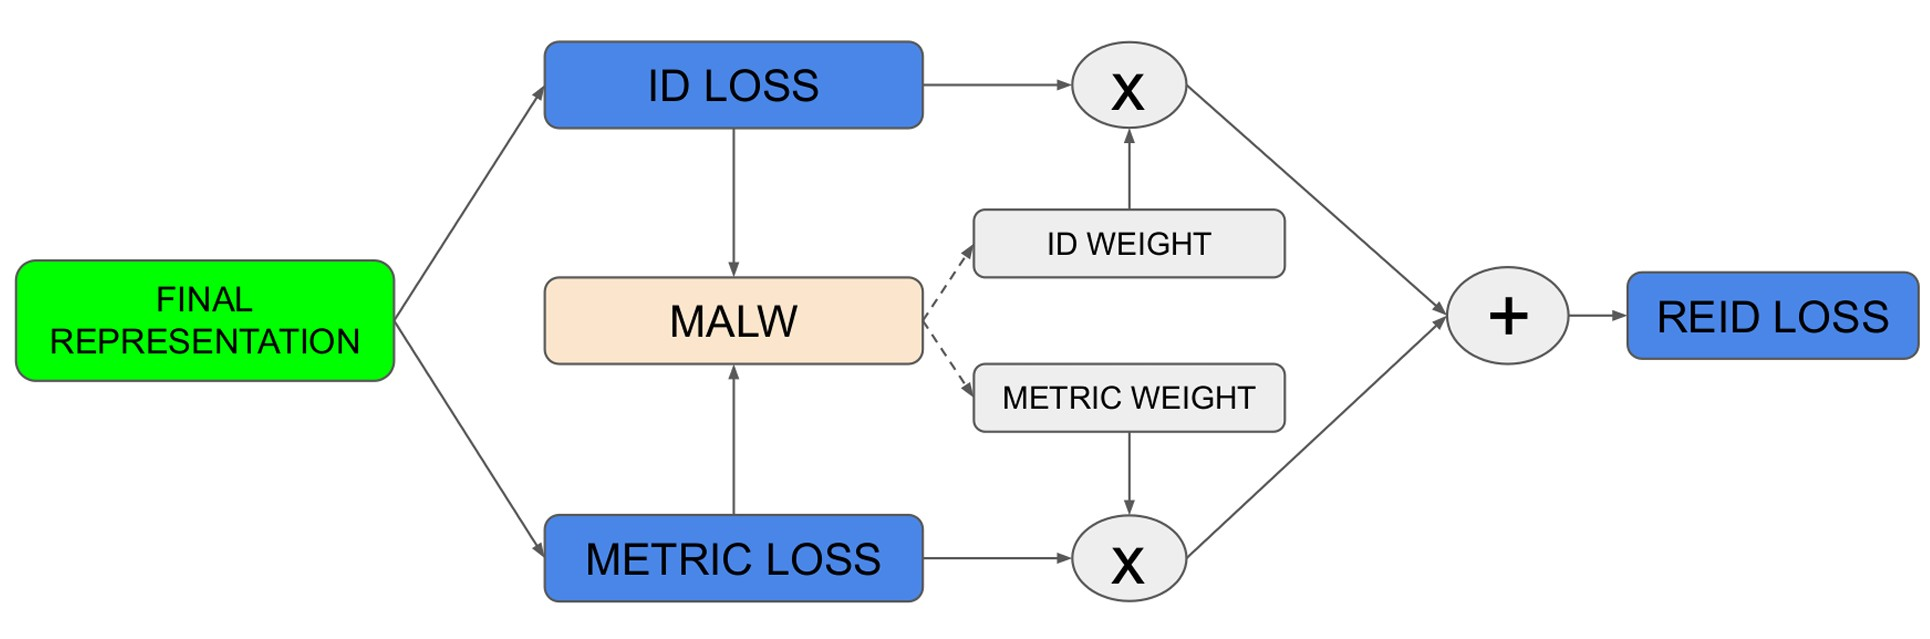
\includegraphics[width=0.8\textwidth]{images/MALW.jpg}
    \caption[Momentum Adaptive Loss Weighting (MALW) Scheme]{Momentum Adaptive Loss Weighting (MALW) Scheme}
    \label{fig:MALW}
\end{figure}

\subsubsection{RPTM Loss}
One of the key challenges in deep metric learning, especially in person or Vehicle Re-Identification tasks, is to optimize the triplet loss effectively since the selection of triplets during training plays a very important role in determining the stability and convergence of the model. Improper triplet selection can lead to either trivial triplets (resulting in no learning) or highly difficult triplets (leading to unstable gradients).

To address this issue, Ghosh et al. (2023) \cite{RPTMLoss} propose a novel triplet selection approach called \textit{Relation-preserving Triplet Mining}, which aims to stabilize the optimization process by a feature matching guided triplet-mining scheme, which ensures that triplets will respect the natural appearance groupings within each ID class. The authors formalize this through a relational indicator $C(x_i, x_j)$ between two instances, defined as:
\begin{equation}
    C(x_i, x_j) = \begin{cases}
    1, & \mathrm{if\ } x_i, x_j \mathrm{\ share\ a\ natural\ subset}, \\
    0, & \mathrm{otherwise}.
    \end{cases}
\end{equation}
RPTM uses feature matching to help establish triplets, leveraging the so called Feature Matcher \textbf{Grid-Based Motion Statistics (GMS)}, which outperforms traditional methods like SIFT, SURF and ORB.
The GMS feature matcher approximates this relational indicator by quantifying the innate relationship between images. Specifically, GMS performs feature matching between an anchor image and potential positive samples within the same ID class, using coherence-based validation to ensure reliable matches across viewpoint changes while minimizing false matches. Authors adopt a semi-hard positive mining strategy: the positive instance is selected based on a threshold $\tau$ set to the average number of GMS matches between the anchor and other images sharing the same ID. In this way, the anchor-positive pairs are not too similar - otherwise, it would lead to trivial learning - and not too dissimilar, which may lead to unstable training as well.

The triplet loss is then modified to incorporate this relation-preserving constraint:
\begin{equation}
L_{tri}(x_a, x_p, x_n) = \max(0, d_{ap} - d_{an} + \alpha)
\end{equation}
where $(x_a, x_p, x_n)$ forms a triplet only if $C(x_a, x_p) = 1$ and $C(x_a, x_n) = C(x_p, x_n) = 0$, ensuring that the anchor-positive pair shares natural appearance characteristics while the negative sample does not. This approach effectively prevents the network from trying to force instances from different natural groups (e.g., front and rear views of a vehicle) to map to the same location in the embedding space, leading to more stable training and better generalization.

\subsection{Dataloaders, Schedulers and Augmentation}
\subsubsection{Dataloader Sampling}
\label{subsubsec:DataloaderSampling}
Under the paradigm of Dataloader Sampling, two leading approaches are often followed: \textit{Random Sampling} \cite{TripletLossV2, EfficientBaseline} and \textit{Balanced Identity Sampling}.

In \textbf{Random Sampling}, for composing a batch $\mathcal{B}$, $P$ identities are randomly sampled from the dataset $\mathcal{D}$ and, for each sampled identity, $K$ images are sampled. This involves having a total batch size of $P \cdot K$ images. However, the serious disadvantage of this strategy is that there could be an identity imbalance, with some identities being sampled more frequently than others, which would affect the generalization performance of the model.

Some methodologies have been suggested to overcome this problem, such as \textit{Hard Mining}. In these approaches, the efforts are concentrated on the selection of hard or problematic instances, mroe specifically in those for which the performance of the model is very poor. By exposing the Optimizer to these challenging samples, the model is driven to improve its learning capabilities, therefore favoring convergence rates and overall efficiency.

Among them, \textit{Batch Hard (BH)} sampling has been one of the most effective approaches in this regard and has performed very well in the literature. It guarantees to select the hardest positive and negative samples from a given batch. More precisely, for every anchor sample in a batch, the hardest positive sample and the hardest negative are chosen. They are the hardest positive and hardest negative, respectively, meaning the one with the largest distance from the anchor and the one with the smallest distance to the anchor. This way, this strategy ensures that the Triplet Loss is focused on those most challenging instances critical for effective training. Concluding, as explained by Hermans et al. \cite{TripletLossV2}, this approach focuses on selecting the hardest samples in every mini-batch, rather than searching through the entire dataset, which saves a lot of computational time.

Another strategy is the \textit{Batch All (BA)} sampling, which estimates the loss across all possible triplets in a batch, therefore considering easier and harder examples. It indeed captures more general relationships but usually incorporates too many triplets that give low contribution to the total loss and hence achieving a slower convergence speed.

These samplings, in particular hard mining, develop unique features that enable the model to become powerful in re-identification tasks.

In this regard, the \textbf{Balanced Identity Sampling} is more elaborated for solving the problem of identity imbalance achieved in the very early stages of Random Sampling. The whole process ensures that every batch is balanced in $P$ identities with $K$ samples per identity. This will avoid overfitting on a few identities while neglecting all the other identities. For this to happen, the Sampler, each time it needs to extract samples, chooses images across cameras or different conditions and if there are not enough instances, it duplicating some samples to make sure all batches are consistent in their number of elements.

\subsubsection{Warmup and Learning Rate Scheduler}
\label{subsubsec:WarmupScheduler}
An important enhancement in the Re-ID training process, is the implementation of a learning rate scheduler with a warm-up phase \cite{BagOfTricks}. The learning rate is increased during the first epochs by the scheduler in a controlled and precise manner, providing a smooth transition into training. This helps avoid abrupt weight updates that may destabilize the optimization strategy in its early stages. After the warm-up, the scheduler will decay to ensure convergence toward an optimal solution. Different decay strategies can be used, such as the \textit{Linear}, \textit{Smooth}, \textit{Multi-Step} or \textit{Cosine} one, which have been proven to be effective in Re-ID tasks.

\subsubsection{Data Augmentation}
Additionally, data augmentation techniques are very popular and proved to be efficient for enhancing generalization by increasing the model's robustness against various different conditions. Popular augmentation strategies are Resize, Random Cropping, Horizontal Flipping, Color jittering, Color Augmentation, Padding, Normalization, and Random Erasing. These techniques and especially the Random Erasing one proved to be very effective in Re-ID tasks, as shown in \cite{BagOfTricks, RandomErasing}.

In detail, Random Erasing is a powerful augmentation technique that strengthens the model's ability to learn robust features. It selects a rectangular region of an image randomly and replaces the pixel values with random noise or a blank/colored patch. This process simulates occlusions, which are common in real-world scenarios; thus, this improves the model's performance handling such conditions. Mathematically speaking, for a given image $I$, the probability of applying Random Erasing Augmentation (REA) is $p$, while the probability of not applying REA is $1-p$. In practice, a patch of dimensions $W \times H$ is randomly selected within the image $I$, where $W$ and $H$ are determined based on the predefined scale range $[s_{\text{min}}, s_{\text{max}}]$ and aspect ratio range $[\text{r}_{\text{min}}, \text{r}_{\text{max}}]$. Concretely, the area of the erased region is uniformly sampled within the total image area within the scale range and the width-to-height ratio of the patch is uniformly sampled within the aspect ratio range, and the pixel values within this patch are set to a constant value $v$, for example, 0, or random noise. Random Erasing performs the desired diversification of occlusions in training by using different scales and aspect ratios for the erased region, which makes the model more robust to partial occlusions encountered in real-world applications, repeating this process for each image in the batch $\mathcal{B}$.

\subsection{Object Detection and Tracking}
The pipeline for multi-camera tracking is divided logically into two parts: MTSC (Multi-Target Single-Camera Tracking) and MTMC (Multi-Target Multi-Camera Tracking), each of these designed to be effective in re-identification of vehicles. The pipeline starts with processing videos or image sequences for each camera given as input. For every camera, or actually for every video, the user may pre-process the video/images by extracting a Region Of Interest (ROI) mask, necessary for focusing the process of detection just on the desired region of interest itself, which essentially is the area where vehicles are supposed to appear. Further steps involve Object Detection, Tracking, Filtering, Feature Extraction, and Similarity Computation.

As for the Object Detection and Tracking phase, the YOLO detector detects vehicles frame-by-frame. The YOLO Detector is able to extract the bounding boxes, classes, IDs and confidence scores of the detected vehicles within the frame, which are then fed into its own Tracker, which updates and maintains a list of active tracks, each of which represents a unique vehicle in the scene. Tracking, instead, is done to keep the same IDs for every detected vehicle, always in frame-by-frame fashion. The tracker associates detections with existing tracks, initiates new tracks for unassociated detections, and updates the state of each track. The tracker will be designed to handle occlusions, appearance changes, and other challenges that may arise during tracking. Overall, its main purpose is to track every vehicle continuously so that each car would keep the same identity between frames in a video.

An extensive hyperparameter search on the Tracker parameter has been conducted to find the best configuration for the tracker. The hyperparameters include the IOU threshold for matching detections to tracks, the maximum number of frames a track can be inactive before being deleted, and the maximum distance between the predicted and detected bounding boxes for a track to be considered active. The Tracker with custom parameters will be denoted as \textbf{Custom} in the evaluation results.
In this study, the tracker type used is \textit{BOTSort}. The following parameters were selected after extensive testing and comparison against default values:

\begin{itemize}
    \item \textit{track\_high\_thresh}: Set to \textbf{0.25} (default: \textbf{0.5}). A lower threshold was chosen to increase the likelihood of associating detections with existing tracks, especially in challenging scenarios with partial occlusions or noisy detections.
    \item \textit{track\_low\_thresh}: Set to \textbf{0.1} (default: \textbf{0.1}). This value was retained as it provides a good balance for secondary association when high-confidence associations are not possible.
    \item \textit{new\_track\_thresh}: Set to \textbf{0.7} (default: \textbf{0.6}). Increasing this threshold reduces the number of false positives when initializing new tracks, ensuring only reliable detections start new trajectories. 
    \item \textit{match\_thresh}: Set to \textbf{0.8} (default: \textbf{0.8}). This parameter was kept at its default value since it effectively balances precision and recall by ensuring that only sufficiently close detections are matched to existing tracks.
    \item \textit{track\_buffer}: Set to \textbf{90} frames (default: \textbf{30}). A longer buffer was selected to allow more frames before deleting inactive tracks, which helps maintain consistent tracking during brief occlusions or missed detections.
\end{itemize}

A proper visualization of the Object Detection, Tracking and ROI management can be appreciated in Figure \ref{fig:ObjDetectionTracking}.

% Object Detection and Tracking Image
\begin{figure}[H]
    \centering
    \includegraphics[width=1.0\textwidth]{images/ObjDetectionTracking.png}
    \caption[Object Detection and Tracking example]{Object Detection and Tracking example. The ROI is the area where vehicles are expected to appear.}
    \label{fig:ObjDetectionTracking}
\end{figure}

The bounding box are converted from the YOLO format (XYWH) to the MOT format (TLWH), which is a standard format used in multi-object tracking datasets, consisting in a list of frame numbers, unique ID, bounding boxes coordinates and other not-so important informations like confidence score. Each vehicle information gets saved in a Python dictionary, which is then appended to a list of dictionaries, representing the vehicles in the scene.

\subsection{Filtering}
\label{subsec:Filtering}
Various filters can be enabled and applied throughout the pipeline in order to enhance data quality, rejecting unwanted data for better detection and tracking accuracy. Filters are applied throughout the pipeline, according to the user's requirements. In practice, usually those filters are activated only when the user is running the pipeline in \textit{Target Mode} and not when evaluating the MTMC phase on the AICity Dataset (\textit{Evaluate Mode}). The following filters are available:

\subsubsection{Stationary vehicle filtering}
The stationary vehicle filter is used to filter vehicles based on their stationary status, improving the quality of the re-identification process and eliminating irrelevant vehicles. This filter is useful in scenarios where the vehicle is parked and remain static for a prolonged period of time, a condition where the tracker will always keep track of it, thus not contributing to a proper multi-camera re-identification process.

The stationary filtering algorithm works by analyzing the movement of the centroid of a vehicle's bounding box across consecutive frames. Let $(x_{t}, y_{t})$ be the centroid of the bounding box at time $t$, and $(x_{t-1}, y_{t-1})$ be the centroid at time $t-1$. The centroids are calculated simply as:
\[
    x_t = tx_t + \frac{w_t}{2}, \quad y_t = ty_t + \frac{h_t}{2}
\]

where \(tx_t\) and \(ty_t\) are the top-left coordinates of the bounding box, and \(w_t\) and \(h_t\) are its width and height, respectively.

Next, the algorithm calculates the frame-to-frame shift of the centroid by computing absolute differences of the \(x\)- and \(y\)-coordinates:

\[
    \Delta x_t = |x_t - x_{t-1}|, \quad \Delta y_t = |y_t - y_{t-1}|
\]

A frame is considered stationary if the movement in both directions is below a predefined threshold \(\tau\) relative to the frame dimensions \(W\) and \(H\):

\[
    \Delta x_t \leq \tau \cdot W, \quad \Delta y_t \leq \tau \cdot H
\]

The algorithm then counts the number of frames in which the vehicle remains stationary. If the total number of such frames exceeds a specified minimum threshold \(M\), the vehicle is classified as stationary and removed from the dataset:

\[
    \verb|stationary_frame_count| > M \implies \verb|remove_vehicle(ID)|
\]

This will filter out the vehicles which are either stationary or running very slowly, which are irrelevant for re-identification across multiple cameras. The two most important parameters here are the stationary threshold \( \tau \) and minimum stationary frame count \( M \), that are tuned to make a good trade-off between the sensitivity of the filter and the error of removing slowly moving vehicles. An example is illustrated in Figure \ref{fig:StationaryFiltering}.

% Stationary Filtering Image
\begin{figure}[H]
    \centering
    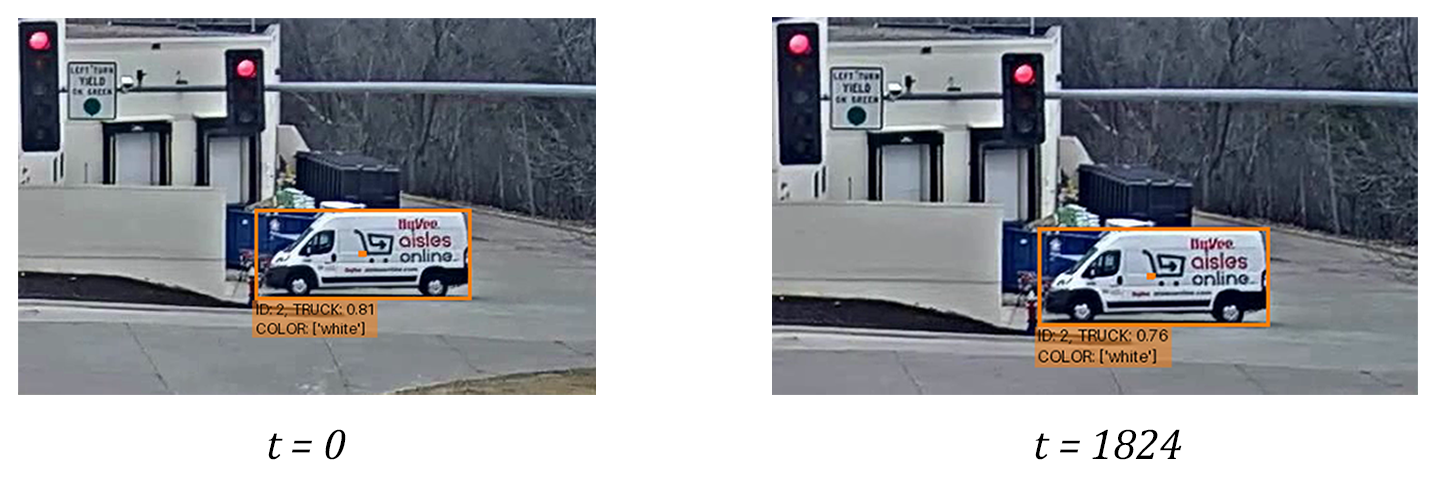
\includegraphics[width=1.0\textwidth]{images/StationaryFiltering.png}
    \caption[Stationary Filtering]{Stationary Vehicle Filtering example. $t$ denotes the current processed frame.}
    \label{fig:StationaryFiltering}
\end{figure}

\subsubsection{Incomplete Bounding Box Filtering}
To further enhance the robustness of the re-identification process, incomplete or improperly detected bounding boxes are filtered out. These bounding boxes often arise from occlusions, partial visibility of vehicles, or errors in the object detection stage. Removing such incomplete bounding boxes ensures that only high-quality data is passed to subsequent stages.

The filtering procedure starts by iterating over the set of detected frames and determining whether a bounding box should be considered incomplete based on several geometric constraints. Let \((tx, ty, w, h)\) denote the top-left coordinates, width, and height of a bounding box in a frame of dimensions \((W, H)\). The criteria used for determining incompleteness are as follows:

\paragraph{1. Minimum Size Check}
A bounding box is considered incomplete if its width or height falls below a predefined minimum size threshold \(s_{\text{min}}\):

\[
w < s_{\text{min}} \quad \text{or} \quad h < s_{\text{min}}
\]

\paragraph{2. Boundary Check}
To avoid including bounding boxes that extend beyond the visible frame area, a margin \(m\) is defined, and the bounding box is considered incomplete if any part of it lies outside the valid region:

\[
tx < m \quad \text{or} \quad ty < m \quad \text{or} \quad tx + w > (W - m) \quad \text{or} \quad ty + h > (H - m)
\]

\paragraph{3. Central Region Check}
Bounding boxes are expected to be located within a central region of the frame, defined by a central threshold \(\tau_{\text{center}}\). The bounding box centroid \((cx, cy)\) is calculated as follows:

\[
cx = tx + \frac{w}{2}, \quad cy = ty + \frac{h}{2}
\]

The bounding box is considered incomplete if its centroid lies outside the central region defined by the limits:

\[
\frac{\tau_{\text{center}}}{2} \cdot W < cx < \left(1 - \frac{\tau_{\text{center}}}{2}\right) \cdot W, \quad \frac{\tau_{\text{center}}}{2} \cdot H < cy < \left(1 - \frac{\tau_{\text{center}}}{2}\right) \cdot H
\]

After applying the above checks, frames containing incomplete bounding boxes are filtered out. The algorithm then computes the number of frames removed during this process, which is given by the difference between the initial and final frame counts. The filtering procedure ensures that only well-detected and complete bounding boxes are retained, thereby improving the reliability of subsequent multi-camera re-identification stages. A visual representation of the Incomplete Bounding Box Filtering is shown in Figure \ref{fig:IncompleteBBFiltering}.

% Incomplete Bounding Box Filtering Image
\begin{figure}[H]
    \centering
    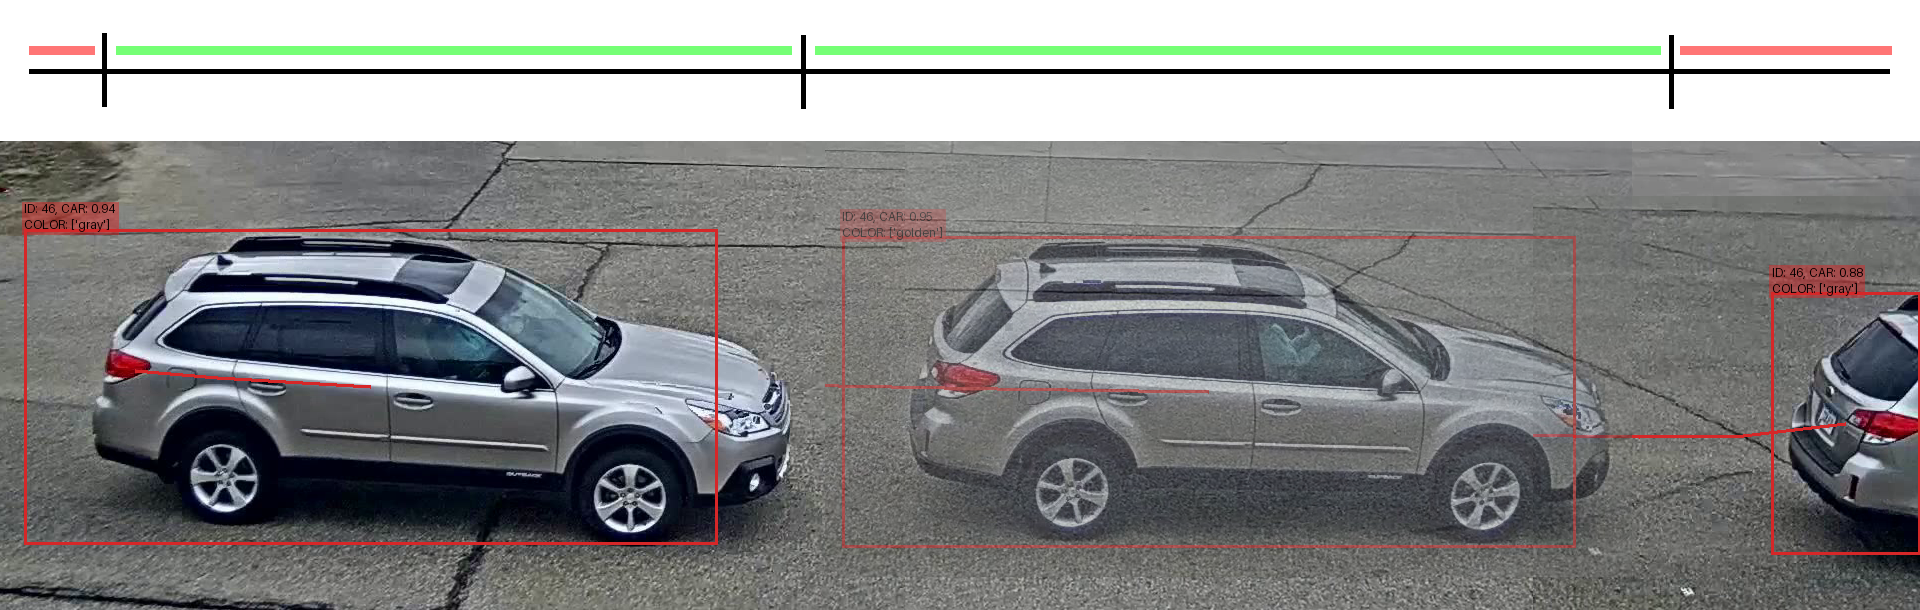
\includegraphics[width=1.0\textwidth]{images/IncompleteFiltering.png}
    \caption[Incomplete Bounding Box Filtering]{Illustration of the incomplete bounding box filtering process. The red and green bar at the top represents frame evaluation: green segments indicate frames with complete bounding boxes that are retained, while red segments indicate frames discarded due to incomplete bounding boxes. Below, bounding boxes are shown around detected vehicles, highlighting which frames passed or failed the completeness check.}
    \label{fig:IncompleteBBFiltering}
\end{figure}

\subsubsection{Color Filtering}
\label{subsubsec:ColorFiltering}
If there are still more frames to process, a color filter can be applied to further refine the dataset. This particular filter eliminates any vehicles not matching an predefined set of target colors. This filter comes in handy in situations when the color of the vehicle is known and the user wants to track only those vehicles of that specific color. This restriction improves the general quality of the Re-ID results, mostly when the process is running, again, in \textit{Target Mode}.

The algorithm starts by checking if the list of target colors $\mathcal{C}_{\text{target}}$ is empty. If no target colors are defined, then the function will terminate early and return the original list of frames. Otherwise, it proceeds with the filtering process based on the color predictions.

Considering a set of frames \(\mathcal{F} = \{f_1, f_2, \ldots, f_N\}\) that corresponds to a specific vehicle identification number, the algorithm further continues to pull the cropped images \(\mathcal{I} = \{I_1, I_2, \ldots, I_N\}\) which depict the detected vehicle in each corresponding frame.

For every image \(I_i \in \mathcal{I}\), the following operations are carried out:
\begin{enumerate}
    \item The image \(I_i\) is converted from an array type to a PIL image.
    \item A transformation function \(T_{\text{val}}\) is applied to prepare the image for inference. This includes resizing, normalization, and conversion to a tensor.
    \item The preprocessed image is then passed through the color classification model.
\end{enumerate}

The color classification model, denoted as $f_{\text{Color}}$, can be one of the following:
\begin{itemize}
    \item A model based on \textbf{EfficientNet} architectures (B3 or B5 variants) where predictions are directly produced as a sequential list of color labels:
    \[
        \text{color\_prediction} = f_{\text{Color}}(I_{i})
    \]
    \item A \textbf{ResNet} architecture integrated with a \textbf{Support Vector Machine} (SVM) classifier. Initially, feature embeddings are obtained via the Re-ID model \(f_{\text{ReID}}\), after which the SVM classifier tries to predict the color:
    \[
        f_{emb} = f_{\text{ReID}}(I_i), \quad \verb|color_prediction| = f_{\text{Color}}(f_{emb})
    \]
\end{itemize}

Regarding the training component for both models, a Multi-Dataset approach combining \textit{VeRi-776} and \textit{VeRi-Wild} datasets has been implemented. The main problem regarding this strategy was the lack of data, hence the creation of a Unified Dataset which combines multiple images and labels from the training set of both datasets. In fact, the unified color classification system harmonizes and deduplicates color labels across both datasets, ensuring consistent color identification across different instances of vehicle datasets. For this matter, a total of 10 color classes were defined, including the most common vehicle colors such as white, black, silver, blue, red, etc. using a total of 300k images were used for training. Another peculiarity of the training process is the choice of the Dataset size. For this reason, the user had the free choice to select the size of the dataset to be used for training, which could range between 1\% and 100\% of the total dataset size. This choice was made to allow the user to train the model with a smaller dataset, which could be useful in case of limited computational resources or time constraints.

The configuration framework employs several key parameters and optimization strategies as the ones followed by the Feature Extraction protocol. Image preprocessing and augmentation strategies were carefully considered. All images undergo standardization to $320 \times 320$ pixels, while maintaining aspect ratios through centered padding rather than aggressive cropping or stretching. The augmentation pipeline includes random horizontal flipping with 0.5 probability as well. Notably, color-based augmentation techniques such as jitter, contrast, and saturation adjustments were intentionally disabled to preserve color fidelity for the classification task.
The training methodology implements a comprehensive loop encompassing both training and validation phases. The loss function utilizes CrossEntropyLoss for classification tasks, while the Adam optimizer handles parameter updates. A particularly significant aspect of the implementation is the sophisticated handling of varying image dimensions. Rather than employing traditional resizing methods that might distort aspect ratios, the system implements a centered padding approach. This methodology preserves the original image proportions while ensuring consistent batch processing capabilities.

Continuing with the filter stage, if the predicted color does not match any of the target colors, the frame is marked for removal, resulting in a final filtered set of frames \(\mathcal{F}_{\text{filtered}}\) for the vehicle ID. The algorithm then calculates the number of frames eliminated during this step by subtracting the original and final number of frames. Color filtering helps the algorithm keep only those vehicles who do match the target colors list, previously defined, thus making the re-identification process of much better quality. An example of the Color Filtering process is depicted in Figure \ref{fig:ColorFiltering}.

% Color Filtering Image
\begin{figure}[H]
    \centering
    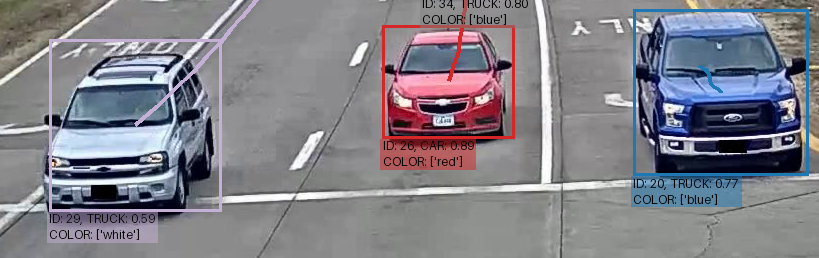
\includegraphics[width=1.0\textwidth]{images/ColorFiltering.png}
    \caption[Color Filtering]{If \(\mathcal{C}_{\text{target}} = ['blue']\), only the right truck, with \(ID = 20\), will be taken into consideration when computing the final re-identification results.}
    \label{fig:ColorFiltering}
\end{figure}

\subsubsection{Minimum frame detection}
Minimum frame detection is a filter that will further refine the frames. The filter can remove those vehicles which are detected for very short durations probably because of false positives or for transient objects. A filter like this will validate only those vehicles which get detected for a number of frames equal or higher than a predefined minimum, hence enhancing the quality in re-identification. It also sets, for every vehicle ID, a global class label, which corresponds to the most frequent class label that the pipeline assigns during the Object Detection phase - avoiding the common little interchanging of class labels between consequent frames.

\subsection{Feature Extraction}
Feature extraction involves the Re-ID model, which will extract the features from the saved frames. The inputs would be the cropped images of the vehicles and, after the inference, a feature vector for each vehicle will be given as output. Actually, the whole methodology followed is very similar to that which has been followed for the color filtering procedure. Feature extraction becomes very important when it comes to the re-identification task since the previously extracted features would then form a basis of comparison for vehicle similarity in diverse cameras, even though that is out of the scope for this subsection.

\subsection{Trajectory Creation}
The trajectory creation process will create a separate trajectory record for each vehicle detected over frames, by properly storing it in a MongoDB database or Pickle files. This step is essential in the Multi-Target Multi-Camera (MTMC) tracking task, as it helps in linking vehicle detections temporally as well as across different camera perspectives.

For every detected vehicle ID, the following steps are performed:

\begin{enumerate}
    \item A \textbf{unique Vehicle ID} is obtained by appending the camera ID with the vehicle ID. It gives an identifier of the form:
    \[
        VehicleID = CAM_{i}\_V_{j}  \quad \text{(e.g., CAM0\_V10)}
    \]
    where \(i\) and \(j\) represent are the camera ID and vehicle ID, respectively.
    \item A corresponding \textbf{Trajectory ID} is created by appending a suffix to the unique vehicle ID:
    \[
        TrajectoryID = CAM_{i}\_V_{j}\_T_{k}  \quad \text{(e.g., CAM0\_V10\_T0)}
    \]
    where \(i, j, k\) represent the Camera ID, Vehicle ID, and Trajectory Index, respectively.
    
    \item Each frame in the sequence undergoes the following processing steps:
    \begin{itemize}
        \item Compression of the cropped vehicle image using an appropriate compression method (\textit{byte-level compression}) in order to save it in MongoDB in an efficient way.
        \item Extraction of the bounding box shape and feature vectors list conversion for efficiency.
        \item Generation of a \textbf{unique bounding box ID} for every frame by appending the frame index as well:
        \[
            BBoxID = CAM_{i}\_V_{j}\_F_{b} \quad \text{(e.g., CAM0\_V10\_F0)}
        \]
        where \(i, j, b\) denotes the camera ID, vehicle ID, and frame index, respectively.
    \end{itemize}

    \item The \textbf{start and end times} of the trajectory are determined from the timestamps of the first and last frames in the sequence.
\end{enumerate}

After the trajectory creation process is done, data is inserted in the MongoDB database. The insertion process consists of the following:

\begin{enumerate}
    \item \textbf{Vehicle Insertion:} Before inserting a new vehicle record, the database is queried to check whether the vehicle already exists. If the vehicle does not exist, a new record is created with its unique ID and class label. The vehicle record is composed by: Vehicle ID and Class Label.
    
    \item \textbf{Bounding Box Insertion:} In every frame, a bounding box record is inserted into the database. If a bounding box with the same ID already exists, the record is updated by incrementing the frame index. The vehicle record is composed by: Frame Index, Bounding Box ID, Bounding Box Shape, Vehicle ID, Compressed Image, Confidence Score, Feature Vector and Timestamp.
    
    \item \textbf{Trajectory Insertion:} The trajectory record, containing the unique trajectory ID, vehicle ID, camera ID, start and end times, is inserted into the database. If the trajectory already exists, it is updated with additional frames. The trajectory record is composed by: Trajectory ID, Vehicle ID, Camera ID, Start Time, End Time.
\end{enumerate}
    
This process, therefore, ensures that the system can handle vehicle tracking in real-time without losing data integrity and by the minimization of redundant entries.

\subsection{Unification}
\label{subsec:Unification}

The unification step tries to enhance the output of the Re-ID pipeline by unifying the set of different vehicle identities that might have been assigned different IDs despite referring to the same physical vehicle. This step is very important in increasing the coherence and accuracy of Multi-Object Tracking and Re-Identification in a single-camera setting. This is precisely shown in Figure \ref{fig:Unification}.

% Unification Image
\begin{figure}[H]
    \centering
    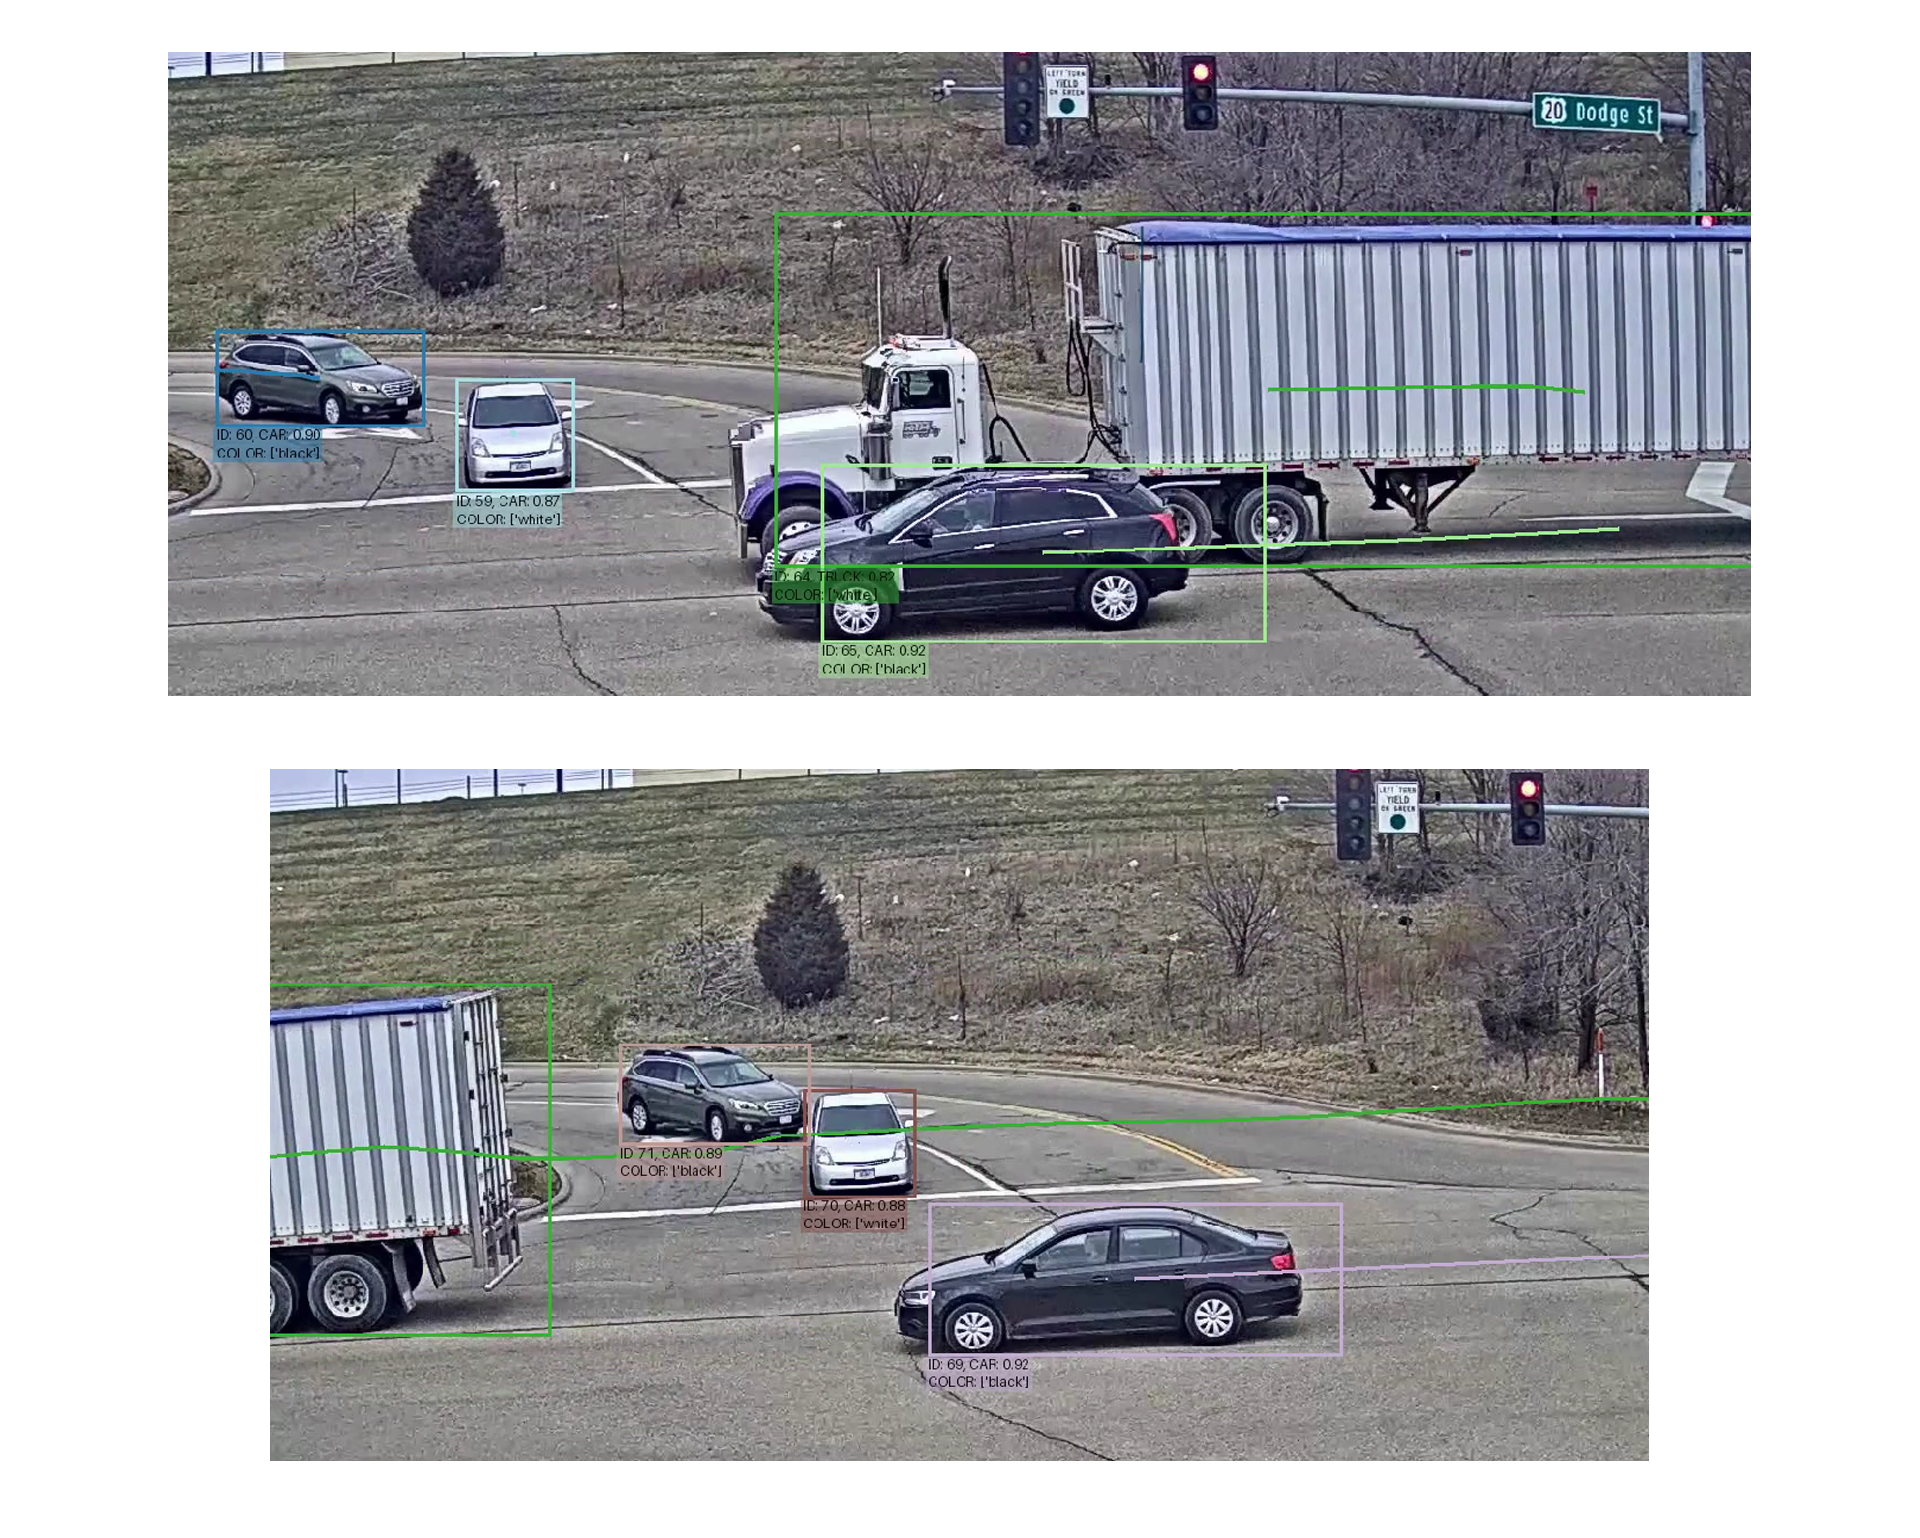
\includegraphics[width=0.90\textwidth]{images/IDSwitch.png}
    \caption[An ID-Switch example]{Unification process. Cars with ID 60 and 59 (top image, left corner) get a mis-assigned ID after the truck with ID 64 passes, as shown in the bottom figure. The unification process aims to merge these IDs into a single one.}
    \label{fig:Unification}
\end{figure}

Once the initial steps in the pipeline - namely, detection and tracking - have been completed, the unification algorithm starts to compute pairwise similarities of features between the vehicles detected by the same camera. Towards this end, an accurate hand-crafted function is adopted that identifies pairs of vehicle IDs with top similarity scores according to multiple unification techniques.
\begin{itemize}
    \item \textbf{Mean Embedding Comparison}: For every vehicle \( v_i \) captured by a camera, the mean embedding is calculated by averaging the feature vectors of all frames associated with that vehicle. Let \( \mathbf{f}_{i}^{(t)} \in \mathbb{R}^{d} \) denote the feature vector of vehicle \( v_i \) at time \( t \), where \( d \) is the dimensionality of the embedding space. The average embedding \( \bar{\mathbf{f}}_{i} \) corresponding to the vehicle \( v_i \) can be expressed as:
    \[
        \bar{\mathbf{f}}_{i} = \frac{1}{T_i} \sum_{t=1}^{T_i} \mathbf{f}_{i}^{(t)}
    \]
    where \( T_i \) denotes the cumulative count of frames in which the vehicle \( v_i \) is present.
    The computation of pairwise similarity \( S(i, j) \) between two vehicles \( v_i \) and \( v_j \) is conducted through the application of cosine similarity, expressed mathematically as follows:
    \[
        S(i, j) = \frac{\bar{\mathbf{f}}_{i} \cdot \bar{\mathbf{f}}_{j}}{\|\bar{\mathbf{f}}_{i}\| \|\bar{\mathbf{f}}_{j}\|}
    \]
    \item \textbf{Individual Frame Comparison}: The similarity of two vehicles is determined by comparing the feature vectors corresponding to their frames individually and then computing the average of the obtained similarities. Let $\mathcal{F}_i$ and $\mathcal{F}_j$ be the sets of feature vectors for vehicles $v_i$ and $v_j$, respectively. The similarity measure $S(i, j)$ between the two vehicles is defined as:
    \[
        S(i, j) = \frac{1}{|\mathcal{F}_i| \cdot |\mathcal{F}_j|} \sum_{\mathbf{f}_p \in \mathcal{F}_i} \sum_{\mathbf{f}_q \in \mathcal{F}_j} \frac{\mathbf{f}_p \cdot \mathbf{f}_q}{\|\mathbf{f}_p\| \|\mathbf{f}_q\|}
    \]
    where $\mid\mathcal{F}_i\mid$ and $\mid\mathcal{F}_j\mid$ denote the number of frames in which vehicles $v_i$ and $v_j$ respectively appear. Such a measure allows finer comparison by examining the similarity of individual frames; it also has the drawback that the computation might take longer since more comparisons need to be done, hence, not suitable for real-time operations.
    \item \textbf{Comparison of Area-Weighted Embeddings}: In this context, each feature vector is assigned a weight that corresponds to the relative area of its associated bounding box. The weight \( w_{i}^{(t)} \) for vehicle \( v_i \) at a given time \( t \) is expressed as follows:
    \[
        w_{i}^{(t)} = \frac{A_{i}^{(t)}}{\min\limits_{t} A_{i}^{(t)}}
    \]
    Here, \( A_{i}^{(t)} \) denotes the bounding box area at time \( t \), which can be formulated as:
    \[
        A_{i}^{(t)} = w_{i}^{(t)} \times h_{i}^{(t)},
    \]
    and \( \min_{t} A_{i}^{(t)} \) denotes the minimum bounding box area across all frames for vehicle \( v_i \).
    The area-weighted average embedding \(\ bar{\mathbf{f}}_{i} \) for the vehicle \( v_i \) is obtained via the following formula:
    \[
        \bar{\mathbf{f}}_{i} = \frac{\sum_{t=1}^{T_i} w_{i}^{(t)} \mathbf{f}_{i}^{(t)}}{\sum_{t=1}^{T_i} w_{i}^{(t)}}
    \]
    Finally, the pairwise similarity \( S(i, j) \) between vehicles \( v_i \) and \( v_j \) is computed using the cosine similarity of their area-weighted mean embeddings:
    \[
        S(i, j) = \frac{\bar{\mathbf{f}}_{i} \cdot \bar{\mathbf{f}}_{j}}{\|\bar{\mathbf{f}}_{i}\| \|\bar{\mathbf{f}}_{j}\|}
    \]
\end{itemize}

After finding the most alike pairs of vehicles, the merging process begins. For each pair $(ID_i, ID_j)$ whose similarity score exceeds a predefined threshold, spatial-temporal constraints are applied:
\begin{itemize}
    \item \textbf{Time Gap Threshold}: The time gap between the last observation of $ID_i$ and the first observation of $ID_j$ has to be less than a predefined maximum threshold.
    \item \textbf{Spatial Distance Threshold}: The Euclidean distance calculated between the centroids of the final bounding box corresponding to $ID_i$ and the initial bounding box associated with $ID_j$ has to be below a predefined range.
\end{itemize}

If both conditions are satisfied, the two tracklets are merged by updating the database entries. In detail, the bounding boxes and the trajectory information belonging to $ID_j$ are assigned to $ID_i$, with $ID_j$ being removed from the database. In addition, if the bounding box images are saved to the local disk (through a specific configuration parameter), the corresponding image files are moved to the folder of $ID_i$.

The unification process can enhance the reliability of the system because it unifies those fragmented tracklets, related to the same vehicle, into a single and coherent identity. It also diminishes the prevalence of redundant identities in a single camera, enhancing its overall Re-ID performance.

\subsubsection{Final Data Export and Storage}
Once all the frames have been processed and the necessary information has been extracted, the final action involves storing the results in a \texttt{.txt} file in a MOTChallenge compliant format.

It all starts by collecting data from the database and by fetching all frames corresponding to a given camera ID. For each vehicle ID, it extracts the frame-level properties, including feature vectors, compressed images, bounding box coordinates, timestamps, and confidence scores. Let \( \mathcal{F} \) be the set of frames of a vehicle \( v \) captured by camera \( c \), where each frame \( f \in \mathcal{F} \) has the following information:
\[
    f = (\mathbf{e}, \mathcal{I}_{\text{comp}}, s, n, b, t, \alpha, v)
\]
where:
\begin{itemize}
    \item \( \mathbf{e} \) represents the feature vector,
    \item \( \mathcal{I}_{\text{compressed}} \) denotes the compressed image data,
    \item \( s \) is the shape of the frame,
    \item \( n \) is the frame number,
    \item \( b = (x, y, w, h) \) defines the bounding box in Top-Left Width-Height (\textit{TLWH}) format,
    \item \( t \) is the timestamp,
    \item \( \alpha \) is the confidence score,
    \item \( v \) is the vehicle ID.
\end{itemize}

For each bounding box, the top-left coordinates \((x, y)\), along with width \(w\) and height \(h\) are extracted and written into a \texttt{.csv} file following the MOTChallenge format:
\[
    \text{Row} = (\text{FrameID}, \text{TrackID}, x, y, w, h, \text{Confidence}, X_{\text{world}}, Y_{\text{world}}, Z_{\text{world}})
\]
The confidence score is set to 1 and real-world coordinates \( (X_{\text{world}}, Y_{\text{world}}, Z_{\text{world}}) \) are initialized to -1, as they are not used in this specific pipeline.
These storage paths are generated dynamically based on the camera ID and a predefined global path for proper organization and retrieval of results at different test scenarios.

\subsection{MTMC and Final Clustering Stage}
\label{subsec:MTMC}

The last part of the pipeline includes steps for \textbf{Multi-Target Multi-Camera (MTMC) tracking} and clustering in order to connect trajectories across multiple cameras. The stage allows to unify the tracks of the same vehicle seen by cameras at different views to a coherent single trajectory.

\subsubsection{Cross-Camera Analysis Setup}
The process begins by loading the \textit{Camera Layout}, which contains spatial and temporal information about the cameras, including their locations and their relative mutual compatibility. The system ensures that vehicles appearing in compatible cameras, meaning cameras which have overlapping FOVs and with overallping time intervals, can be considered for linking.

Some key cross-camera spatial and temporal calibrations will be pursued with the help of the \textit{Camera Layout} itself. Some major parameters are shown as follows:
\begin{itemize}
    \item \textbf{FPS (Frames per Second)}: Frame rate of the cameras.
    \item \textbf{Scales}: An array of multiplicative factors which is used for normalizing the time values across the different cameras.
    \item \textbf{Offsets}: Temporal offsets to bring cameras to a common and synchronized starting time.
    \item \textbf{Compatibility Matrix}: A binary matrix indicating whether two cameras have overlapping fields of view, hence they are compatible.
    \item \textbf{Transition Windows} (\(\text{dt}_{\min}\) and \(\text{dt}_{\max}\)): Minimum and maximum time intervals allowed for a vehicle to transition between cameras.
\end{itemize}

The \textbf{scales} and \textbf{offsets} parameters serve to adjust small temporal differences between cameras when linking tracklets. As different cameras may have slight variations in recording speed or starting times, these parameters align events properly across the multi-camera setup.
The scale for a given camera \(i\) is computed as:
\[
    \text{scale}_i = \frac{t_{2}}{t_{1}}
\]
where \(t_{1}\) and \(t_{2}\) are the times taken for the same event to occur on the reference camera and camera \(i\), respectively.

Similarly, the offset for a camera \(i\) is given by:
\[
    \text{offset}_i = t_{1} - t_{2}
\]
where \(t_{1}\) and \(t_{2}\) are the appearance times of the same vehicle in the beginning of the video on the reference camera and camera \(i\), respectively.

The vehicle tracklets are collected either from a precomputed \textit{Pickle} file or directly from the database, depending on the configuration. Each tracklet includes frames, bounding boxes, timestamps, and extracted features.

\subsubsection{Tracklet Construction}
For each camera, tracklets are constructed using the collected frames from the DB or the Pickle files.
Each tracklet will include:
\begin{itemize}
    \item \textbf{Vehicle ID}, which indicates the unique ID of the vehicle.
    \item \textbf{Mean Feature}, computed as the average of the frame features. Necessary for globally representing the tracklet.
    \item \textbf{Start and End Times}, derived from the timestamps of the first and last frames. More precisely, Camera parameters come into play, since the $\textit{global}$ start and end times of each tracklet is being computed. For a tracklet \( \text{track} \) in camera \(i\) with local start time \(t_{\text{start}}\) and end time \(t_{\text{end}}\), the global times are computed as:
    \[
    T_{\text{start}} = \frac{t_{\text{start}}}{\text{fps}_i \cdot \text{scale}_i} + \text{offset}_i
    \]
    \[
    T_{\text{end}} = \frac{t_{\text{end}}}{\text{fps}_i \cdot \text{scale}_i} + \text{offset}_i
    \]
\end{itemize}
This information is very important for the successive clustering and merging process.

\subsubsection{Similarity Matrix Computation}
The similarities between all tracklets are computed based on their mean features. For two tracklets $\text{track}_1$ and $\text{track}_2$ with their respective mean features $\mathbf{f}_1$ and $\mathbf{f}_2$, the similarity score $s$ is computed as the dot product:
\[
s = 
\begin{cases}
\mathbf{f}_1 \cdot \mathbf{f}_2, & \text{if already normalized} \\
\frac{\mathbf{f}_1 \cdot \mathbf{f}_2}{\|\mathbf{f}_1\|_2 \|\mathbf{f}_2\|_2}, & \text{otherwise}
\end{cases}
\]
When a different \textbf{linkage} method is given (such as \textit{average}, \textit{single}, or \textit{complete}), the similarity is computed by retrieving pairwise similarities from a precomputed similarity matrix \( \mathbf{S} \):
\[
    \textbf{average: } s = \frac{1}{|T_1| \cdot |T_2|} \sum_{t_1 \in T_1, t_2 \in T_2} S[t_1, t_2]
\]
\[
    \textbf{single: } s = \max_{t_1 \in T_1, t_2 \in T_2} S[t_1, t_2]
\]
\[
    \textbf{complete: } s = \min_{t_1 \in T_1, t_2 \in T_2} S[t_1, t_2]
\]

\subsubsection{Track Merging}
The two conditions below must be satisfied to merge the tracklets:
\begin{itemize}
    \item \textbf{Compatibility}: The tracklets belong to physically compatible cameras separated by an overlap of time intervals. Two cameras are compatible if their time intervals intersect a boundary condition, like:
    
    Compatible if:
    \[ T_{2, \text{start}} \leq T_{1, \text{end}} + \delta_{t_{\max}} \quad \text{and} \quad T_{2, \text{end}} \geq T_{1, \text{end}} + \delta_{t_{\min}} \]
    or viceversa:
    \[ T_{1, \text{start}} \leq T_{2, \text{end}} + \delta_{t_{\max}} \quad \text{and} \quad T_{1, \text{end}} \geq T_{2, \text{end}} + \delta_{t_{\min}} \]
    where \( \delta_{t_{\min}} \) and \( \delta_{t_{\max}} \) are the minimum and maximum time intervals allowed for a vehicle to transition between cameras.
    \item \textbf{Similarity}: The tracklets must have a similarity score greater than a threshold (\( \theta_{\text{sim}} \)).
\end{itemize}

\subsubsection{A Priority Queue for Track Merging}
A \textbf{priority queue} is utilized to manage merging tracklets across cameras. This priority queue contains candidate pairs of tracklets to be merged sorted in descending order by their similarity scores. Each entry in the queue will be represented as:
\[
    \text{Entry} = (-\text{similarity}, \text{timestamp}, \text{track}_i, \text{track}_j)
\]
here, negative similarity implements a \textit{max-heap}, so pairs with highest similarity will be first processed.

The similarity between two tracklets is computed as the dot product between their normalized mean feature vectors:
\[
    \text{similarity}(\text{track}_i, \text{track}_j) = \frac{\mathbf{f}_i \cdot \mathbf{f}_j}{\|\mathbf{f}_i\|_2 \|\mathbf{f}_j\|_2}
\]
where \(\mathbf{f}_i\) and \(\mathbf{f}_j\) denote the mean feature vectors of the two tracklets.

To speed up the computation of similarity, all mean features are stacked into a matrix \(\mathbf{F}\), and the similarity matrix is computed by a matrix multiplication:
\[
    \mathbf{S} = \mathbf{F} \cdot \mathbf{F}^\top
\]

This technique exploits GPU acceleration with \texttt{torch}, thus reducing the time complexity relative to pairwise dot products. Next, once the similarity matrix has been computed, there is a collection of tracklets, which are appended to the priority queue for further merging based on the similarity score above a given threshold.

During merging, if a pair of tracklets are spatially and temporally compatible, they will be merged and the similarity matrix is updated. The above procedure proceeds until there are no more compatible pairs in the priority queue. In other words, the pipeline itself performs an incremental merging of tracklets depending on their visual similarities but certainly also taking into consideration motion constraints.

\subsubsection{Final Prediction Output}
Once the merging process is complete, the final consolidated trajectory will thus be saved in the \textbf{MOTChallenge format}. For each camera, the system then generates a prediction file containing:
\begin{itemize}
    \item Frame number
    \item Track ID
    \item Bounding box coordinates (in \textit{TLWH} format)
    \item Confidence score
\end{itemize}
A \textit{Pickle} file is also generated containing the final tracklets with their corresponding frames and features for further analysis.

\subsection{Target Mode}
The pipeline, as previously teased, can operate in \textit{Target Mode}, which means that the user would like to track a particular vehicle of interest in a series of various camera views. In this specific operating mode, the pipeline will not compute the MTMC metrics corresponding to the AICity Dataset; instead, it takes as input a reference picture of the target vehicle and a corresponding camera ID which specifies from which the picture has been taken. The system, therefore, utilizes the same Deep Learning-based Re-ID features used in the MTMC clustering step to find the most similar vehicle instances across the entire camera network immediately after the MTMC pipeline has successfully been executed (i.e., meaning just after the Trajectory Creation step and the Final Clustering phase).

The target vehicle identification can be done by one of the following three ways:

\begin{itemize}
    \item \textbf{Multi-track Search}: This method is first performed aggregating the vehicle detections into a complete trajectory and then comparing the target vehicle with the average feature embeddings of each trajectory. With the intent of thereby avoiding false positives, it specifically excludes any trajectory starting from the same camera as the target vehicle and, in particular, focuses on the inter-camera matches. The similarity is then computed using normalized feature vectors which returns the top-K most similar trajectories. Overall, this method employs the MTMC final clustering trajectories to access the most comparable occurrences of the target vehicle across different cameras.
    \item \textbf{Single-track Search}: This is even more accurate and detailed as it provides better comparisons of the target vehicle against single vehicle tracks rather than whole trajectories. It can be used effectively in cases of partial or fragmented trajectories because it assesses each track individually without requiring a complete trajectory reconstruction. Again, just like the others, trajectories from the same camera are also excluded. 
    \item \textbf{Camera-link Search}: The most advanced method is to construct trajectories incrementally between cameras. It will start with finding the optimal matches in the first camera, and from there it will progressively connect to the next most similar vehicle in the following cameras. This method performs best in consistent identity across the entire camera network since it uses spatial links among the cameras.
    All three methods are based on the same Re-ID model which produce stable and reliable features for the target vehicle.
    The feature extraction for the Target Vehicle is similar to the others, while the similarity is calculated through the same cosine similarity measure. The system generates a ranked list of potential matches, which allows the user to view the most probable examples of the target vehicle from different camera views. This feature is of special value in applications like law enforcement, traffic monitoring, or analysis of vehicle movement patterns in an urban environment. An example is shown in Figure \ref{fig:TargetSearch}.
\end{itemize}

% Target Mode Image
\begin{figure}[H]
    \centering
    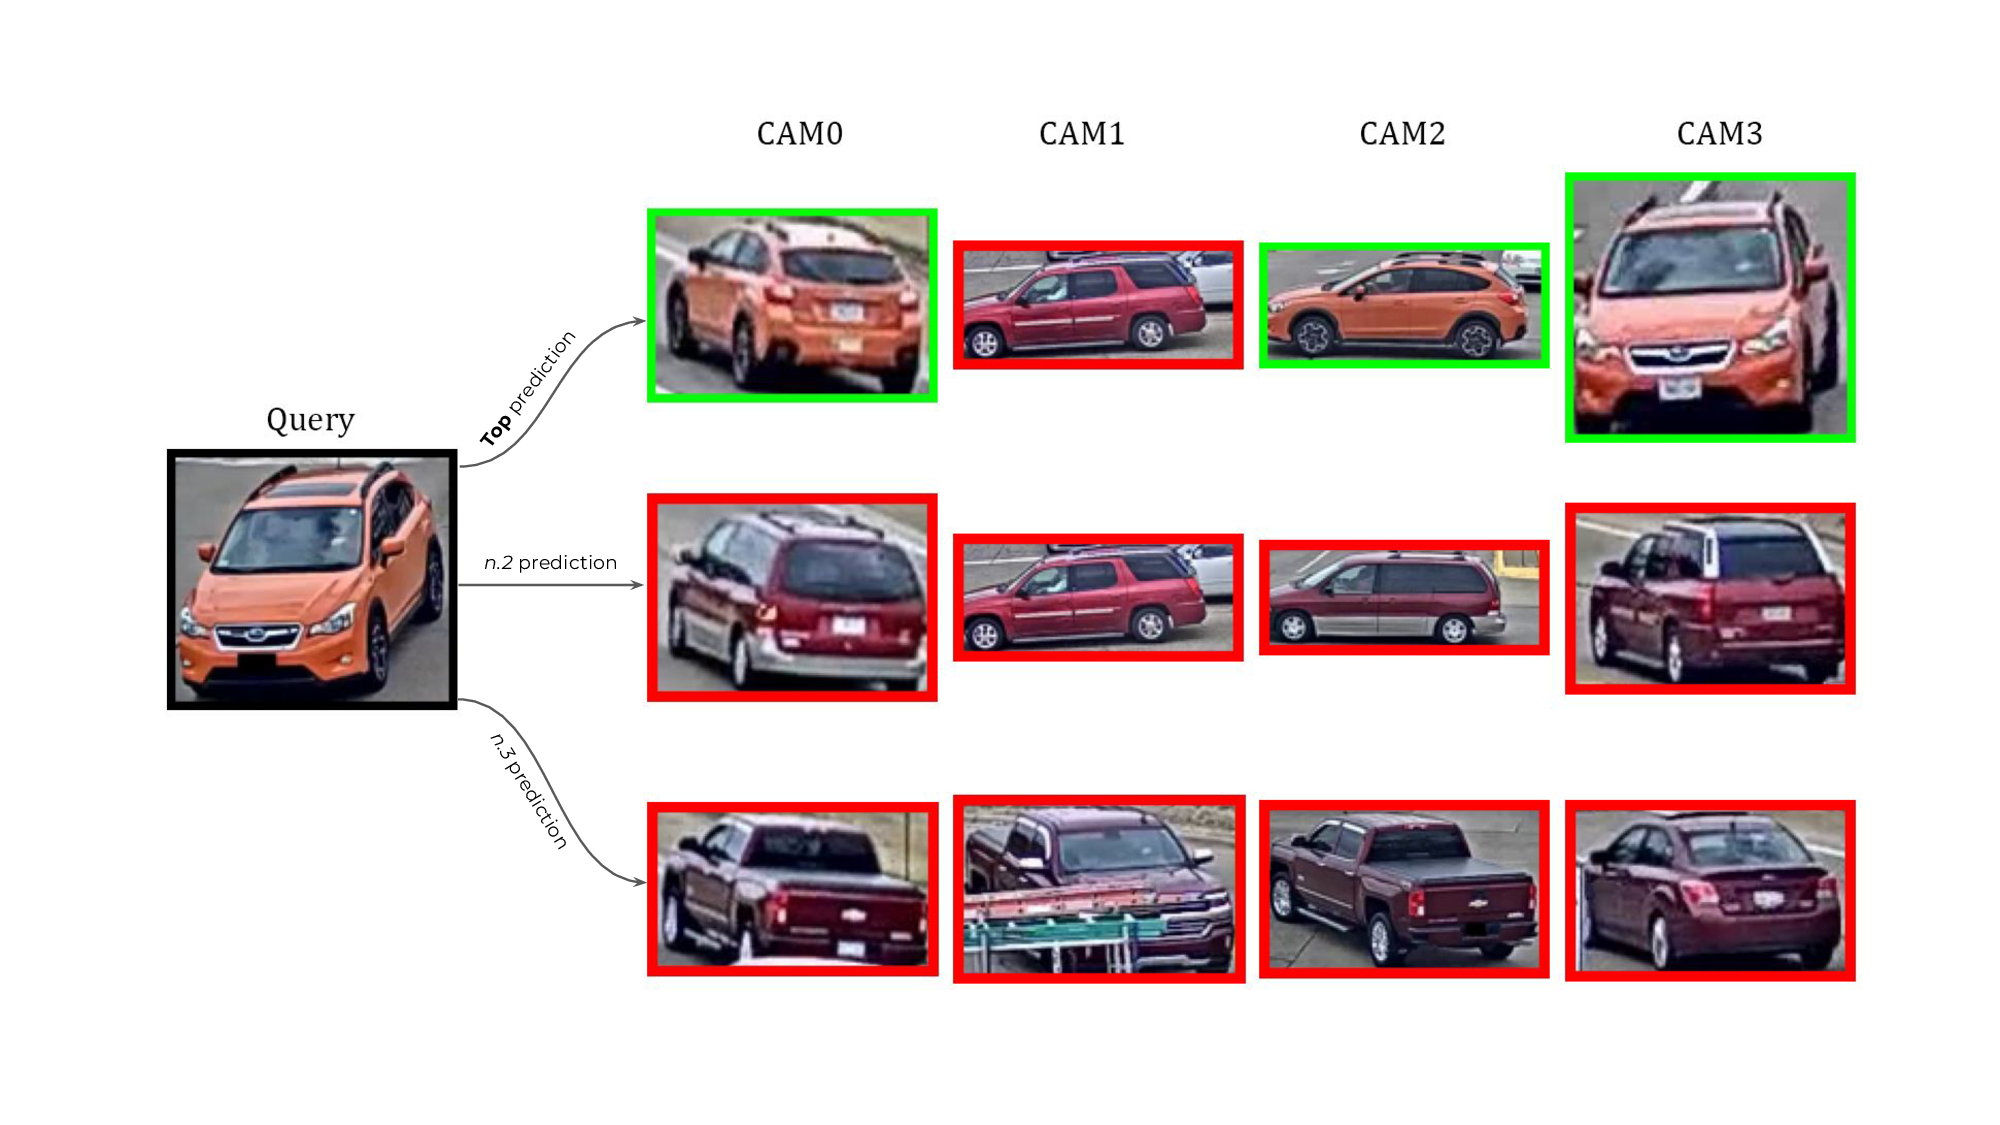
\includegraphics[width=1.0\textwidth]{images/TargetSearch.png}
    \caption[Target Search Results]{An example of the Target Mode search. In this example, the first row denotes the top-result coming from the pipeline. The Target Vehicle is not present in first row - Camera 1 because it passes below the camera view FOV, hence it's not present in the overall system.}
    \label{fig:TargetSearch}
\end{figure}

% Pipeline Overview Image
\begin{figure}[ht]
    \centering
    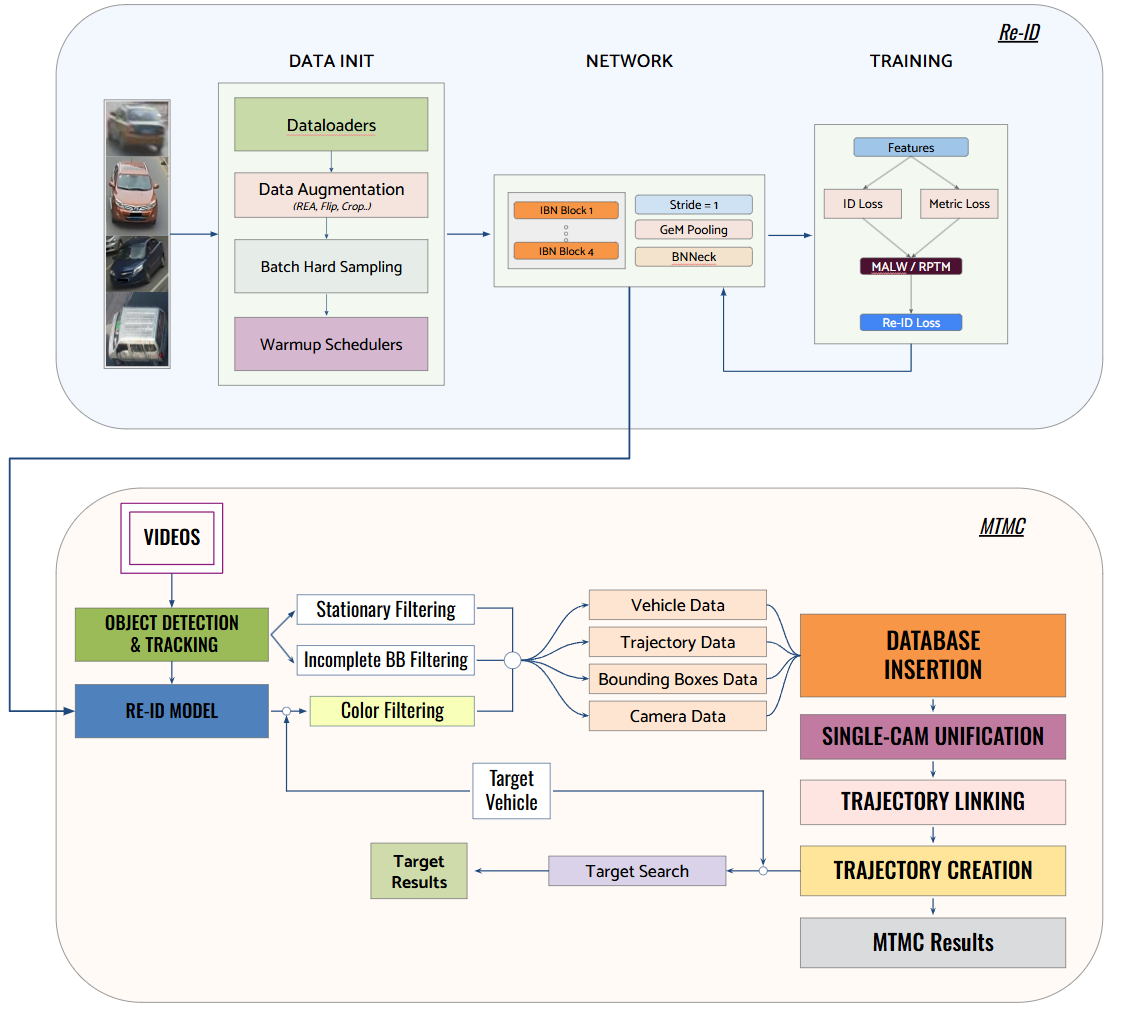
\includegraphics[width=1.0\textwidth]{images/PipelineOverview.png}
    \caption[Pipeline overview]{Pipeline Overview. The pipeline consists of several stages, including Re-ID Training, Object Detection, Tracking, Filtering, Feature Extraction, Trajectory Creation, Unification and MTMC Final Tracking. Color filtering is only applied in Target Mode.}
    \label{fig:PipelineOverview}
\end{figure}
